
\chapter{Identifying multi-locus chromatin contacts in human cells using tethered multiple 3C}

\graphicspath{{11_tmc/}}

\begin{work}
This chapter has been published in a slightly modified form in
\citet{ay:identifying}, as joint work with Ferhat Ay, Thanh H. Vu, Michael J.
Zeitz, Jan E. Carette, Jean-Philippe Vert, Andrew R. Hoffman and William S. Noble.
\end{work}

\begin{abstract}{Abstract}

\textbf{Background:} Several recently developed experimental
methods, each an extension of the chromatin conformation capture (3C)
assay, have enabled the genome-wide profiling of chromatin contacts
between pairs of genomic loci in 3D. Especially in complex eukaryotes,
data generated by these methods, coupled with other genome-wide
datasets, demonstrated that non-random chromatin folding correlates
strongly with cellular processes such as gene expression and DNA
replication.

\textbf{Results:} We describe a genome architecture assay, tethered
multiple 3C (TM3C), that maps genome-wide chromatin contacts via a
simple protocol of restriction enzyme digestion and religation of
fragments upon agarose gel beads followed by paired-end sequencing. In
addition to identifying contacts between pairs of loci, TM3C enables
identification of contacts among more than two loci simultaneously.
We use TM3C to assay the genome architectures of two human cell lines:
KBM7, a near-haploid chronic leukemia cell line, and NHEK, a normal
diploid human epidermal keratinocyte cell line.  We confirm that the
contact frequency maps produced by TM3C exhibit features
characteristic of existing genome architecture datasets, including the
expected scaling of contact probabilities with genomic distance,
megabase scale chromosomal compartments and sub-megabase scale
topological domains.  We also confirm that TM3C captures several known
cell type-specific contacts, ploidy shifts and translocations, such as
Philadelphia chromosome formation (Ph+) in KBM7.  We confirm a subset
of the triple contacts involving the \emph{IGF2-H19} imprinting
control region (ICR) using PCR analysis for KBM7 cells.  Our
genome-wide analysis of pairwise and triple contacts demonstrates
their preference for linking open chromatin regions to each other and
for linking regions with higher numbers of DNase hypersensitive sites
(DHSs) to each other.  For near-haploid KBM7 cells, we infer whole
genome 3D models that exhibit clustering of small chromosomes with
each other and large chromosomes with each other, consistent with
previous studies of the genome architectures of other human cell
lines.

\textbf{Conclusion:} TM3C is a simple protocol for ascertaining genome
architecture and can be used to identify simultaneous contacts among three
or four loci. Application of TM3C to a near-haploid human cell line
revealed large-scale features of chromosomal organization and multi-way
chromatin contacts that preferentially link regions of open chromatin.

\textbf{Keywords:} genome architecture, chromatin conformation capture,
multi-locus chromatin contacts, near-haploid human cells, leukemia,
three-dimensional modeling.

\end{abstract}

\section*{Background}

A variety of microscopic imaging techniques have long been used to study
chromatin architecture and nuclear organization
\citep{langer-safer:immunological, manders:four-dimensional,
cremer:multicolor}. Recent advances triggered by the invention of chromatin
conformation capture (3C) enable ascertainment of genome architecture on a
genome-wide scale for virtually any genome, including human
\citep{lieberman-aiden:comprehensive, dixon:topological, jin:high-resolution},
mouse \citep{zhang:spatial, dixon:topological}, budding yeast
\citep{duan:three}, bacteria \citep{umbarger:three-dimensional}, fruit fly
\citep{sexton:three-dimensional} and a malarial parasite
\citep{ay:three-dimensional}. These studies have revealed that the
three-dimensional form of the genome {\em in vivo} is highly related to genome
function through processes such as gene expression and replication timing.
Therefore, understanding how chromosomes fold and fit within nuclei and how
this folding relates to function and fitness is crucial in gathering a
thorough picture of epigenetic control of gene regulation for eukaryotic
organisms.


Hi-C was the first molecular assay to measure genome architecture on a genome-wide
scale \citep{lieberman-aiden:comprehensive}, and the assay continues to
be widely used \citep{jin:high-resolution, naumova:organization, ay:three-dimensional}.
Hi-C involves seven steps: (1) crosslinking cells with
formaldehyde, (2) digesting the DNA with a six-cutter restriction enzyme, (3)
filling overhangs with biotinylated residues, (4) ligating the fragments, (5)
creating a sequence library using streptavidin pull-down, (6) high-throughput
paired-end sequencing, and (7) mapping paired ends independently to the genome
to infer contacts. A subsequently described assay by \citet{duan:three} is more
complex, involving a pair of restriction enzymes (REs) applied in three separate
steps (RE1, RE2, circularization, then RE1 again), as well as the introduction
of EcoP151 restriction sites to produce paired tags of 25--27bp. More recently,
the tethered conformation capture (TCC) assay enhances the signal-to-noise
ratio by carrying out a Hi-C-like protocol using DNA that is tethered to a
solid substrate \citep{kalhor:genome}.

One limitation of current genome architecture assays is their
inability to identify simultaneous interactions among multiple
loci. Chromosomes are composed of complex higher order chromatin
structures that bring many distal loci into close proximity.  In
particular, evidence suggests that eukaryotic transcription occurs in
factories containing many genes \citep{cook:organization}.
Recently, multiple-gene
interaction complexes associated with promoters were found to contain
an average of nearly nine genes \citep{li:extensive}. However, currently
available experimental data cannot ascertain to what extent these
multiple gene interactions occur simultaneously or are confined to
different sub-populations of nuclei. This distinction is analogous to
the distinction between ``party hubs'' and ``date hubs'' in
protein-protein interaction networks, in which a hub protein interacts
either simultaneously or in a serial fashion with a series of partner
proteins~\citep{han:evidence}. In the context of genome architecture assays,
distinguishing between ``party loci'' and ``date loci'' will be a
crucial first step in elucidating the role of combinatorial regulation
of gene expression.

{
A molecular colony technique recently developed by \citet{gavrilov:quantitative}
investigated multicomponent interactions
among remote enhancers and active $\beta$-globin genes in
mouse erythroid cells. This assay, however, is PCR-based and requires a
primer design step, which prevents it from providing a genome-wide
picture of potential multicomponent contacts. An earlier genome-wide
assay by Sexton et al., which is adapted from the traditional Hi-C protocol and
is similar to the assay we present here, acknowledged the existence
of multi-locus contacts that can be identified from paired-end reads
in their data \citep{sexton:three-dimensional}.
However, due to a number of differences in that
protocol compared to TM3C (e.g., size selection for larger fragments,
shorter read lengths and no in-gel ligation step), identifying a
substantial number of multi-locus contacts was not possible when we
apply our two-phase mapping pipeline to the Sexton et al.\ data
($<$0.0004\% triples and no quadruples). Therefore, genome-wide methods
that distinguish between simultaneous contacts among multiple loci and
pairwise contacts that happen in different sub-populations of cells
are still necessary.
}
\begin{figure}
\centering
\includegraphics[width=1.0\textwidth]{figs/Figure1.pdf}
\caption{
\textbf{Overview of TM3C experimental protocol and mapping of paired-end reads to human genome.}
  {\bf 1.} Cells are treated with
  formaldehyde, covalently crosslinking proteins to one another and to
  the DNA. The DNA is then digested with either a single 4-cutter
  enzyme (DpnII) or a cocktail of enzymes (AluI, DpnII, MspI, and
  NlaIII). {\bf 2.} Melted low-melting agarose solution is added to
  the digested nuclei to tether the DNA to agarose beads.  Thin
  strings of the hot nuclei plus agarose solution is then transferred to an
  ice-cold ligation cocktail overnight. {\bf 3.} After reversal of
  formaldehyde crosslinks and purification via gel extraction, the
  TM3C molecules are sonicated and size-selected for 250 bp fragments.
  {\bf 4.} Size-selected fragments are paired-end sequenced (100 bp per end)
  after addition of sequencing adaptors.
  {\bf 5.} Each end of paired-end reads are mapped to human reference genome.
  If both ends are mapped then the pair is considered a \emph{double} and retained
  because it is informative for genome architecture.
  {\bf 6.} Read ends that do not map to the reference genome are identified
  and segregated according to the number of cleavage sites they contain for
  the restriction enzyme(s) used for digestion.
  {\bf 7.} Reads with exactly one cleavage site are considered for the second
  phase of mapping. These reads are split into two from the cleavage site and
  each of these two pieces are mapped back to the reference genome.
  {\bf 8.} Read pairs with either one or both ends not mapped in the first
  mapping phase are reconsidered after second phase. Depending on how many
  pieces stemming from the original reads are mapped in the second phase,
  such pairs lead to either no informative contacts, \emph{doubles},
  \emph{triples} or \emph{quadruples}.
}
\label{fig:outline}
\end{figure}


To address this issue, we developed the tethered multiple chromosome
conformation capture assay (TM3C), which involves a simple protocol of
restriction enzyme digestion and religation of fragments within agarose gel
beads (tethering step) followed by high throughput paired-end sequencing
(Figure~\ref{fig:outline}, steps 1--4). We apply TM3C to two human cell lines
and confirm that the DNA--DNA contact matrices produced by TM3C exhibit
features characteristic of existing genome architecture datasets, including
the expected scaling of contact probabilities with genomic distance,
enrichment of intrachromosomal contacts, megabase scale chromosomal
compartments and sub-megabase scale topological domains. We confirm that TM3C
in KBM7 cells captures several known cell type-specific contacts, ploidy
shifts and translocations, such as Ph+ formation. In addition, we demonstrate
that TM3C enables genome-wide identification of contacts among more than two
loci simultaneously. We identify multi-locus contacts involving three (triple)
or four (quadruple) loci by a two-phase mapping strategy that separately maps
chimeric subsequences within a single read (Figure~\ref{fig:outline}, steps
5--8). This mapping strategy potentially allows us to identify co-regulation
or combinatorial regulation events, while also greatly increasing the number
of distinct pairwise contacts (doubles) identified. We also validate a subset
of the triple contacts involving the \emph{IGF2-H19} imprinting control region
(ICR) using PCR for KBM7 cells. We demonstrate that pairwise and triple
contacts prefer to link open chromatin regions to each other and regions with
higher numbers of DHSs to each other.
%Furthermore, we show that our triple contacts are enriched among loci that
%contain enhancers and/or promoters as annotated in the six Tier 1 ENCODE cell
%lines~\citep{hoffman:integrative}.
Finally, we use the contact maps gathered from TM3C to infer a local 3D
structure of the \emph{IGF2-H19} region at 40~kb resolution and a whole genome
3D model at 1~Mb resolution for the near-haploid KBM7 genome. Our 3D models
place \emph{H19} and \emph{IGF2} genes far away from each other, consistent
with their opposite transcriptional status, and place gene-rich small
chromosomes (chrs.\ 16, 17, 19--22) and large chromosomes (chrs.\ 1--5) near
each other, confirming previous observations of gene-density-correlated
arrangements of higher-order chromatin in human cells~\citep{bolzer:three}.

%%%% Results start %%%%%
%%%%%%%%%%%%%%%%%%%%%%%%
\section*{Results}

\subsection*{Tethered multiple chromatin conformation capture (TM3C)}
To identify simultaneous chromatin contacts among two or more loci,
we digest crosslinked chromatin with one or more 4-cutter restriction
enzymes (REs) (Step 1 of Figure~\ref{fig:outline}). When using multiple
REs, we select a set of enzymes such that sticky or blunt ends left by one
enzyme are incompatible with the ends left by any other, thereby preventing
ligation between fragments generated by different enzymes. We then encapsulate
and ligate the digested DNA within agarose beads
(Step 2 of Figure~\ref{fig:outline}), which replaces the tethering step of
\citet{kalhor:genome}. We then size-select DNA fragments of around 250~bp
and subject the selected fragments to high throughput paired-end sequencing
(Steps 3, 4 of Figure~\ref{fig:outline}). Our assay differs from the original
Hi-C assay in three primary ways: (i) TM3C can use multiple REs simultaneously,
(ii) TM3C does not include a step where sticky ends of restriction fragments
are biotinylated, and (iii) TM3C carries out the ligation step within agarose
gel beads. Digestion using multiple REs greatly increases the resolution that
can be achieved via these genome-wide 3C-based techniques
(Supplementary Fig.~\ref{suppfig:cutSiteComparison}). However, comparison of
two libraries, one generated with four 4-cutters and the other with only one,
suggests that the noise-to-signal ratio is much higher for the multiple 4-cutters case.
Our second modification, elimination of the biotinylation step, greatly reduces
the complexity of the overall protocol and has already been applied successfully by
\citet{sexton:three-dimensional}. This simplification, however,
comes with the drawback of sequencing many uninformative, unligated sonication
products both for the TM3C and the Sexton et al.\ protocols. Because detection of
such uninformative read pairs is computationally trivial, this simplification,
fortunately, does not contribute an additional noise factor. The third
modification we implement, in-gel ligation, is similar to but simpler
than the tethering achieved
using protein biotinylation in the tethered conformation capture (TCC)
assay \citep{kalhor:genome}. Our initial experimental data which omitted
the in-gel ligation demonstrated that without this step the resulting
signal-to-noise ratio for the case of four 4-cutters is very low
(95\% of the contacts are interchromosomal). Addition of in-gel ligation step
improved the percentage of intrachromosomal contacts from 5\% to 20\% and
48\% for the four 4-cutter (KBM7-TM3C-4) and one 4-cutter (KBM7-TM3C-1)
libraries, respectively. Therefore, we only present the results from the
libraries generated using the in-gel ligation and focus mainly on the
results from our one 4-cutter library for both KBM7 and NHEK cell lines.

We use TM3C to investigate the chromatin architecture of the near haploid cell
line KBM7 (25, XY, +8, Ph+) extracted from a heterogeneous chronic leukemia
cell line~\citep{kotecki:isolation}, and NHEK, a normal diploid human keratinocyte primary cell
line (Lonza Walkersville Inc.). We construct libraries using only one four-base cutter restriction enzyme
(TM3C-1) for both KBM7 and NHEK. We also create two libraries from KBM7
cells using four different four-base cutters, one from crosslinked cells (KBM7-TM3C-4)
and one from non-crosslinked cells (KBM7-MCcont-4) as a control (Table~1). In what follows,
we report results from application of TM3C to these two human cell lines mainly
focusing on KBM7.

\subsection*{TM3C reveals multi-locus chromatin contacts}

\begin{figure}
  \centering
  \subfloat[KBM7]{\label{fig:noOfREsites}\includegraphics[width=0.37\textwidth]{figs/noOfCutSites.pdf}}
  \hspace{0.01\textwidth}
  \subfloat[]{\label{fig:distScaling}\includegraphics[width=0.28\textwidth]{figs/intraChrScaling/allLibs.pdf}}
  \hspace{0.01\textwidth}
  \subfloat[KBM7]{\label{fig:logScaling}\includegraphics[width=0.30\textwidth]{figs/intraChrScaling/KBM7-100bp-TMC-1.pdf}}
  \vspace{0.02\textheight}
  \\[-\lineskip]
  \subfloat[KBM7-TM3C-1]{\label{fig:KBM7TMC1heatmap}
    \includegraphics[width=0.4\textwidth]{figs/interchrHeatmaps/heatmaps-beforeNormalization/KBM7-100bp-TMC-1.pdf}}
    \hspace{0.05\textwidth}
  \subfloat[KBM7-TM3C-4]{\label{fig:KBM7TMC4heatmap}
    \includegraphics[width=0.4\textwidth]{figs/interchrHeatmaps/heatmaps-beforeNormalization/KBM7-100bp-TMC-4.pdf}}
    \vspace{0.02\textheight}
  \\[-\lineskip]
  \subfloat[NHEK-TM3C-1]{\label{fig:NHEKTMC1heatmap}
    \includegraphics[width=0.4\textwidth]{figs/interchrHeatmaps/heatmaps-beforeNormalization/EK43-100bp-TMC-1.pdf}}
    \hspace{0.05\textwidth}
  \subfloat[KBM7-MCcont-4]{\label{fig:KBM7MCcontheatmap}
    \includegraphics[width=0.4\textwidth]{figs/interchrHeatmaps/heatmaps-beforeNormalization/KBM7-100bp-MCcont-4.pdf}}
\caption{
\textbf{Consistency of TM3C data with known organizational principles and KBM7 karyotype.}
{\bf(a)} Number of RE cut sites within reads that are fully mapped and
nonmapped in the first phase mapping for KBM7 libraries.
{\bf(b)} Scaling of contact probability with genomic distance for three
crosslinked libraries and one non-crosslinked control library.
{\bf(c)} Scaling of contact probability in log--log scale for three different
sets of contacts identified in KBM7-TM3C-1 library.
Pairwise chromosome contact matrices for
{\bf(d)} KBM7-TM3C-1, {\bf(e)} KBM7-TM3C-4,
{\bf(f)} NHEK-TM3C-1 and {\bf(g)} KBM7-MCcont-4 libraries. For these plots
contact counts are averaged over all pairs of mappable 1~Mb windows between the
two chromosomes.
}
\label{fig:validation}
\end{figure}
\clearpage



In addition to providing higher resolution, the use of frequently cutting REs
(4-cutters) or multiple REs together allows identification of simultaneous
contacts among more than two loci, even with reads as short as
100~bp.
The original Hi-C method only retains read pairs in which
both reads map completely to the reference genome. Here we refer to
this type of contacts as type \textbf{F-F} (fully mapped/fully mapped,
Step 5 of Figure~\ref{fig:outline}). Unlike current Hi-C mapping
pipelines, after identifying {\bf F-F}
pairs, we further process the unmapped paired-end reads to see whether we can still
rescue some informative chromatin contacts from them. Our motivation to pursue
these reads stems from the striking difference between the number of restriction
sites within fully-mapped versus non-mapped reads
(Figure~\ref{fig:validation}a). In both the TM3C-1 and TM3C-4
libraries, greater than 70\% of the
non-mapped reads contain at least one RE cut site,
whereas 90\% of the mapped reads contain no cut sites for the TM3C-1 library
(two sample Kolmogorov-Smirnov test p-values for both TM3C-1 and TM3C-4 are approximately equal to 0).
This difference
suggests that read ends that fail to map as a whole can still be informative of
chromatin contacts because they potentially contain real ligation events leading
to chimeric reads. In order to extract this contact information, we further process
the read ends containing one restriction site, thereby identifying contacts
between a partially mapped read and a fully mapped read (\textbf{P-F})
or between two partially mapped reads (\textbf{P-P}, Steps 6--8 of
Figure~\ref{fig:outline}, Methods). This two-phase
mapping strategy not only identifies a
greater number of pairwise contacts (doubles) but also allows
us to identify contacts involving three or four loci from only one paired-end read.
Step 8 of Figure~\ref{fig:outline} summarizes the different cases arising from the second
mapping phase for a read pair that did not qualify as {F-F} in the
first phase. Overall, after excluding intrachromosomal contacts with
genomic distance $<$20~kb, we identify more than 210K triples from our KBM7-TM3C-1
library together with 10.1M and 857K additional pairwise contacts from {P-F}
and {P-P} type read pairs, respectively (Table~2, Additional file 2).
We also investigate the mapping orientations (signs) of ligated fragments that
create different contact types (Table~3). The distribution of reads among all possible
sign combinations is expected to have a bias for reads that are sonication products
(undigested or religated) and to be uniform for de novo chromatin contacts due
to ligation events. Table~3 shows this is the case for both the contacts that are
identified by traditional Hi-C pipelines (F-F) as well as for the contacts we identify
here that produce triples. Since we size select for fragments that are
approximately 250~bp, the
genomic distance threshold of 1~kb eliminates all sonication products, resulting
in uniform distribution for the remaining contacts from TM3C.


\subsection*{Two-phase mapping rescues contacts informative of genome architecture}
Following identification of all three types of contacts (F-F, P-F, and
P-P), we evaluate the quality
of the resulting contact sets for each library in four ways. First, we confirm that the contact
probability between two intrachromosomal loci exhibits a sharp decay with increasing
genomic distance for crosslinked libraries but not for the control library
when all contact types are pooled (Figure~\ref{fig:validation}b). Second, we
observe that this scaling relationship is consistent for different contact
types (Figure~\ref{fig:validation}c),
and the scaling is log-linear for the genomic distance range of 0.5--7~Mb, consistent with
observations from Hi-C data \citep{lieberman-aiden:comprehensive}. Third, we
confirm visually and quantitatively that the interchromosomal contact maps
we obtain from each contact type are consistent with each other
(Supplementary Fig.~\ref{suppfig:compareThreeTypes}, pairwise matrix correlations
are 0.997, 0.964 and 0.954 for (F-F, P-F), (F-F, P-P) and (P-F, P-P), respectively)
and that the contact maps are consistent with known organizational hallmarks
of human genome architecture, such as the increased number of contacts between
small chromosomes (16--22 except 18) (Figure~\ref{fig:validation}d--f, Supplementary Fig.~\ref{suppfig:compareThreeTypes}).
Fourth, we confirm that our contact profiles capture known karyotypic abnormalities
of KBM7 cells, such as diploidy of chromosome 8 (+8), partial diploidy of chromosome 15,
and t(9;22)(q34;q11)) translocation between chromosomes 9 and 22 that leads to
Philadelphia chromosome formation~\citep{kotecki:isolation,burckstummer:reversible}
(Figure~\ref{fig:validation}d, e, Supplementary Fig.~\ref{suppfig:KBM7ploidyTrack}).
Normal diploid human keratinocyte (NHEK) cells exhibit no karyotypic abnormalities
except higher average contact counts between chromosomes 17, 19 and 22
(Figure~\ref{fig:validation}f).
For the non-crosslinked KBM7 control library, only the changes related to copy number
(e.g., diploidy) are apparent from the heatmap (Figure~\ref{fig:validation}g).  Translocations are not visible
in the control because digestion of non-crosslinked chromatin does not preserve genomic distances.
Together, these results indicate that TM3C successfully assays genome architecture
of human cells and suggests that contacts recovered by our two-phase mapping strategy, which are
traditionally discarded from Hi-C analysis, are consistent with traditionally
retained contacts. Therefore, for all remaining analyses with pairwise contacts
we combine all three types (F-F, P-F, P-P) into an aggregated contact map for each library.

\subsection*{TM3C data confirms chromatin compartments and topological domains}
{

\begin{figure}
  \centering
  \subfloat[KBM7]{\label{fig:KBM7eigChr17}\includegraphics[width=0.4\textwidth]{figs/KBM7-100bp-TMC-1-chr17.pdf}}
  \hspace{0.05\textwidth}
  \subfloat[GM06990~\citep{lieberman-aiden:comprehensive}]
  {\label{fig:GM3eigChr17}\includegraphics[width=0.4\textwidth]{figs/Lieberman_human_GM-12-chr17.pdf}}
  \vspace{0.02\textheight}
  \\[-\lineskip]
  \subfloat[KBM7]{\label{fig:KBM7tdChr6}\includegraphics[width=0.4\textwidth]{figs/KBM7-100bp-TMC-1-chr6-topDomains.pdf}}
  \hspace{0.05\textwidth}
  \subfloat[IMR90~\citep{dixon:topological}]{\label{fig:IMR90tdChr6}\includegraphics[width=0.4\textwidth]{figs/hIMR90-chr6-topDomains.pdf}}
\caption{
\textbf{Figure 3 - Comparison of TM3C data with existing genome architecture datasets}
Eigenvalue decomposition to identify open/closed chromatin compartments of
chromosome 17 {\bf(a)} from the KBM7 cell line assayed by TM3C and {\bf(b)}
from GM06990 cell line assayed by Hi-C~\citep{lieberman-aiden:comprehensive}.
Topological domain calls and contact count heatmaps of a 6 Mb region of chromosome 6
{\bf(c)} for the KBM7 cell line assayed by TM3C and {\bf(d)} for the
IMR90 cell line assayed by Hi-C~\citep{dixon:topological}.
}
\label{fig:cellLineComparison}
\end{figure}


In addition to evaluating whether results from the TM3C data sets are consistent with
polymer models of chromatin folding and karyotypic properties of assayed cell lines,
we assess whether TM3C contact maps exhibit the expected compartment-scale and domain-scale
organization. For this purpose we perform eigenvalue decomposition on our
contact maps and compare our compartment calls to those of previous Hi-C data sets
on other human cell lines~\citep{lieberman-aiden:comprehensive,dixon:topological}.
The resulting compartment calls exhibit a nearly perfect overlap for chromosome 17
between KBM7 and GM06990 (Figures~\ref{fig:cellLineComparison}a--b)
and a high level
of genome-wide conservation (82$\%$) between these two cell lines. Conservation
between pairs of contact maps from the five previously published contact maps
ranged between 70--82\%.

Similarly, we perform topological domain decomposition at 40~kb resolution on
KBM7 contact maps and compare our calls to those of two human cell lines
published by \citet{dixon:topological} (Methods).
Figures~\ref{fig:cellLineComparison}c--d demonstrate the significant overlap of
topological domain calls from KBM7 and IMR90 contact maps on a 12~Mb region of
chromosome 6. Overall, 73\% of IMR90 and 72.8\% of ESC domain boundaries overlap
with the boundaries that we identify for the KBM7 cell line
(Fisher's exact test p-values compared to random overlap are $<10^{-100}$ for each case).
}

Together, the compartment-scale and domain-scale similarities between our data
and previous Hi-C data suggests that TM3C, a simpler protocol, provides similar
results to Hi-C and that KBM7, which has a distinct karyotype, preserves
the large scale organizational features of other human cell lines.

{
\subsection*{Genome-wide characterization of triple contacts}

\begin{figure}
  \centering
  \subfloat[]{\label{fig:TripleComps}\includegraphics[width=0.45\textwidth]{\detokenize{figs/doubleTriple-Comps.pdf}}}
  \hspace{0.05\textwidth}
  \subfloat[]{\label{fig:TripleDHS}\includegraphics[width=0.45\textwidth]{\detokenize{figs/doubleTriple-DHS.pdf}}}
%  \vspace{0.05\textwidth} \newline
%  \subfloat[]{\label{fig:TripleEP}\includegraphics[width=1.0\textwidth]{\detokenize{figs/doubleTriple-EP.pdf}}}
\caption{
\textbf{Figure 4 -  Genome-wide characterization of triple contacts}
{\bf(a)} Observed over expected percentages of double and triple contacts that
 link 1~Mb regions with the same (either open or closed) or different (mixed)
 compartment labels for the KBM7-TM3C-1 library (Methods). Both double and triple
 contacts prefer to link open compartments to each other with triples showing slightly
 more enrichment for this trend.
 {\bf(b)} Similar percentages as in {\bf(a)} but when 1~Mb windows are segregated
 according to the number of DHSs they contain (Methods). Contacts linking regions with
 higher numbers of DHSs than the median number are enriched within the doubles
 and the triples of the KBM7-TM3C-1 library. Due to lack of DNase data
 for KBM7 cells, we use data from six other human cell lines for this analysis.
 Since the results are very similar among different cell lines, here we only plot
 the results for K562 which is also a leukemia cell line.
% {\bf(c)} Observed over expected percentages of triple contacts that link enhancers
% to promoters and promoters to other promoters at 40~kb resolution (Methods).
% We use ENCODE genome segmentations in six human cell lines to extract regions
% annotated as ``enhancers'' and ``promoters'' (Methods)~\citep{hoffman:integrative}.
% For K562 annotations 19.02\% and 5.65\% of all triples contain one enhancer-promoter
% (one E-P) and multiple enhancer-promoter (multi E-P) contacts, respectively.
}
\label{fig:triplesNEW}
\end{figure}


After identifying chromatin compartments at 1~Mb resolution and topological domains
at 40~kb resolution for the KBM7 cell line,
we evaluate whether the triple contacts identified by TM3C preferentially link
regions with the same compartment labels and regions within the boundaries of a
topological domain. Figure~\ref{fig:triplesNEW}a shows that triple contacts,
similar to doubles, are enriched among regions of open chromatin
(observed 14.6\% compared to expected 8.33\%, Methods). Out of all intrachromosomal
triples (triples that link three loci on the same chromosome), we see that 16.5\%
are within the same topological domain. Note that we exclude from this percentage
all short range intrachromosomal triples ($<$20~kb) as well as all those that link
at least two loci within the same 40~kb window which would otherwise inflate the
reported percentage. We assess the significance of this observed percentage of
intradomain triples by generating a null model with 100 shuffled topological
domain decompositions for each chromosome (Methods). The median
and the mean percentages are both $\sim$14.1\% with a standard deviation of 0.16\%
for the null model suggesting a statistically significant enrichment of
intradomain triples for the observed domain decomposition compared to shuffled
configurations (p-value$=0$, z-score$=14.67$).

Next we carry out an analysis similar to the compartment label analysis
described above using the numbers of DNase hypersensitive sites within
each 1~Mb window (Methods). Figure~\ref{fig:triplesNEW}b shows that, consistent
with and slightly surpassing the enrichment for open chromatin compartments,
triple contacts as well as doubles are enriched among regions with higher
numbers of DHSs (for triples observed 23.7\% compared to expected 12.4\%, Methods).

%Last, we test the hypothesis that triple contacts preferentially link regulatory
%elements such as enhancers and promoters to each other. Due to the lack of ChIP-seq
%data to generate these annotations for the KBM7 cell line, we use six other human
%cell lines that have been annotated by ENCODE (Methods)~\citep{hoffman:integrative}.
%We find that our triples are enriched for both single and multiple enhancer-promoter contacts as well as
%promoter-promoter contacts (Figure~\ref{fig:triplesNEW}c). It is important to note that performing this analysis
%at 40~kb resolution we exclude all proximal contacts, which presumably are
%highly enriched for enhancer-promoter interactions. Furthermore, because a substantial
%portion of enhancers are cell type specific, we believe that the enrichments shown
%here represent only a subset of enhancers that are common between the cell line
%of the annotation and KBM7. Indeed, recomputing the enrichments by restricting
%ourselves only to the enhancer and promoter annotations that are common to all
%six cell types results in higher enrichment than in any one cell line for each
%of the four interaction groups (enrichment of 2.08 for multi E-P group compared
%to an average of 1.62 for individual cell lines). These results suggest that the
%genome-wide triple contacts identified by our framework are enriched for interactions
%between regulatory elements, consistent with our hypothesis that they
%are enriched with
%combinatorial regulation events occurring within an individual cell.
}

\subsection*{Verification of triples involving \emph{IGF2-H19} locus}

\begin{figure}
  \centering
  \subfloat[]{\label{fig:ICRtriples}\includegraphics[width=1.0\textwidth]{figs/ICR-triples.pdf}}
  \vspace{0.03\textwidth}
  \subfloat[]{\label{fig:ICRgel}\includegraphics[width=0.55\textwidth]{figs/onlyTriples3and5.pdf}}
\caption{
\textbf{Figure 5 -  Validation of triples using PCR}
{\bf(a)} Ten triples extracted from the KBM7-TM3C-1 library that have at least one of
their three ends in the 40~kb region surrounding the imprinting control region (ICR)
of \emph{IGF2} and \emph{H19} genes.
These triples involve short- and long-range contacts within
chromosome 11 which are all indicated by tick marks with coordinates in kilobases (kb)
displayed only for long-range contacts.
Interchromosomal contacts with other chromosomes are indicated by the chromosome identifier
followed by the coordinate in megabases (Mb). Orientation of the displayed locus is in
the direction of \emph{IGF2} and \emph{H19} transcription.
{\bf(b)} PCR verification of pairwise contacts from triples 3 and 5. One pair
of forward/reverse primers is used for each gel (Supplementary Table~\ref{supptable:PCRprimers}).
}
\label{fig:PCRvalidation}
\end{figure}


%% NOTE: IFG2 is the human version of gene and Igf2 is the mouse one
We next investigate whether the multi-locus contacts identified by the TM3C
assay correspond to possible combinatorial regulatory interactions in
KBM7 cells. Specifically, we focus on triples (contacts involving three loci)
involving the \emph{IGF2-H19} locus, which is a classic example of imprinting that
leads to allele-specific gene expression and regulation in both mouse and
human~\citep{bartolomei:parental, ling:ctcf, vu:loss, murrell:interaction}.
Our previous work in human cells
has shown that a region that is located just upstream of the \emph{H19} promoter
which is differentially methylated between maternal and paternal copies is involved
in formation of allele-specific long-range chromatin loops~\citep{vu:loss}.
Methylation status of this imprinting control
region (ICR) determines whether \emph{IGF2} is transcribed (paternal allele)
or not (maternal allele). Because KBM7 cells are haploid for chromosome 11, we
expect our TM3C data to be consistent with only one mode of operation of
this ICR. Analyzing the triples inferred from KBM7-TM3C-1 data involving
the ICR region ($\pm$20~kb), we observe contacts that link this ICR region
to distal loci on the same chromosome as well as to a {\em trans} loci on
other chromosomes (Figure~\ref{fig:PCRvalidation}a).

In order to verify
these contacts, we design three primers per each triple and perform PCR
experiments (Supplementary Table~\ref{supptable:PCRprimers}).
We test whether pairs of forward/reverse primers give rise to PCR
products with expected sizes to confirm contacts identified from our
two-phase mapping (Figure~\ref{fig:PCRvalidation}b). For triple 3, we use
primers 3a and 3c designed for two loci that are 80~kb away and are linked by a
contact found from a ligation occurring within one end of a paired-end read.
For triple 5, we use primers 5a and 5c that link two loci that are 24 kb
apart on chromosome 11 and are found (one of them only partially) in two
separate ends of a paired-end read. For both of these cases we observe
PCR products near the expected size from our primer design (Supplementary Table~\ref{supptable:PCRprimers}).
Validation of contacts found by our two-phase mapping either within a
single end of a read or from two different ends supports the idea that
chimeric reads contain information about genuine chromatin contacts.

Next, we perform PCR on all the triples shown in Figure~\ref{fig:PCRvalidation}a
using all three primers simultaneously. Out of 10 triples tested, 6 of them
(triples 1--6) resulted in either one or more PCR products that have the
expected size(s), confirming these contacts
(Supplementary Figs.~\ref{suppfig:tenTriples},~\ref{suppfig:only5and6Gels}, Supplementary Table~\ref{supptable:PCRprimers}).
Detailed analysis of the distal loci that are contact partners of ICR
(either interchromosomal or interchromosomal with distance $>$40~kb to ICR)
in these six triples reveal that most of these loci
(6 out of 8, Supplementary Figs.~\ref{suppfig:triple1methyl}--\ref{suppfig:triple3methyl})
lie in regions consisting mainly of unmethylated CpGs in K562 cells and
mainly methylated CpGs in at least one other cell line assayed by ENCODE~\citep{encode:integrated}.
These contacts suggest existence of complex chromatin loops that
bring together the differentially methylated ICR in 3D
with loci that show cell type-specific methylation and specifically
unmethylation in K562 cells. These results together with our preliminary
methylation analysis of the ICR suggest a 3D organization which
silences \emph{IGF2} by restricting enhancer access to its promoter
similar to \emph{Igf2} silencing of the maternal copy of mouse
chromosome 7~\citep{qiu:complex}. In order to test our hypothesis
that the single copy of chromosome 11 in KBM7 corresponds to the
maternal allele, we check the expression status of \emph{H19} and
\emph{IGF2} genes from a recently published data set~\citep{burckstummer:reversible}.
Supplementary Fig.~\ref{suppfig:IGF2expr} shows that \emph{H19}
is expressed but \emph{IGF2} is not as we expected. This expression
data confirms the prediction from TM3C data for the parent-of-origin
of chromosome 11 in KBM7 cells. Furthermore, our 3D model
of the 2~Mb region centered on the ICR (Figure~\ref{fig:3D}a) demonstrate
that the two genes, expressed \emph{H19} and non-expressed \emph{IGF2},
are placed in distal chromatin domains, consistent
with the proposed gene regulation model in the maternal copy of the
homologous region in mouse~\citep{murrell:interaction}. However, the
depth of our data is not sufficient to do a finer scale 3D modeling
that can distinguish between allele specific loops established
by several differentially methylated regions and CTCF binding sites.


\subsection*{Three-dimensional modeling of KBM7 genome recapitulates known organizational principles of human cells}

\begin{figure}
  \centering
  \subfloat[Chromosome 11 1Mb--3Mb]{\label{fig:3Dchr11}\includegraphics[width=0.3\textwidth]{\detokenize{figs/Nelle-3D/KBM7-IGF2-3D.pdf}}}
   \hspace{0.06\textwidth}
  \subfloat[All chromosomes]{\label{fig:3Dall}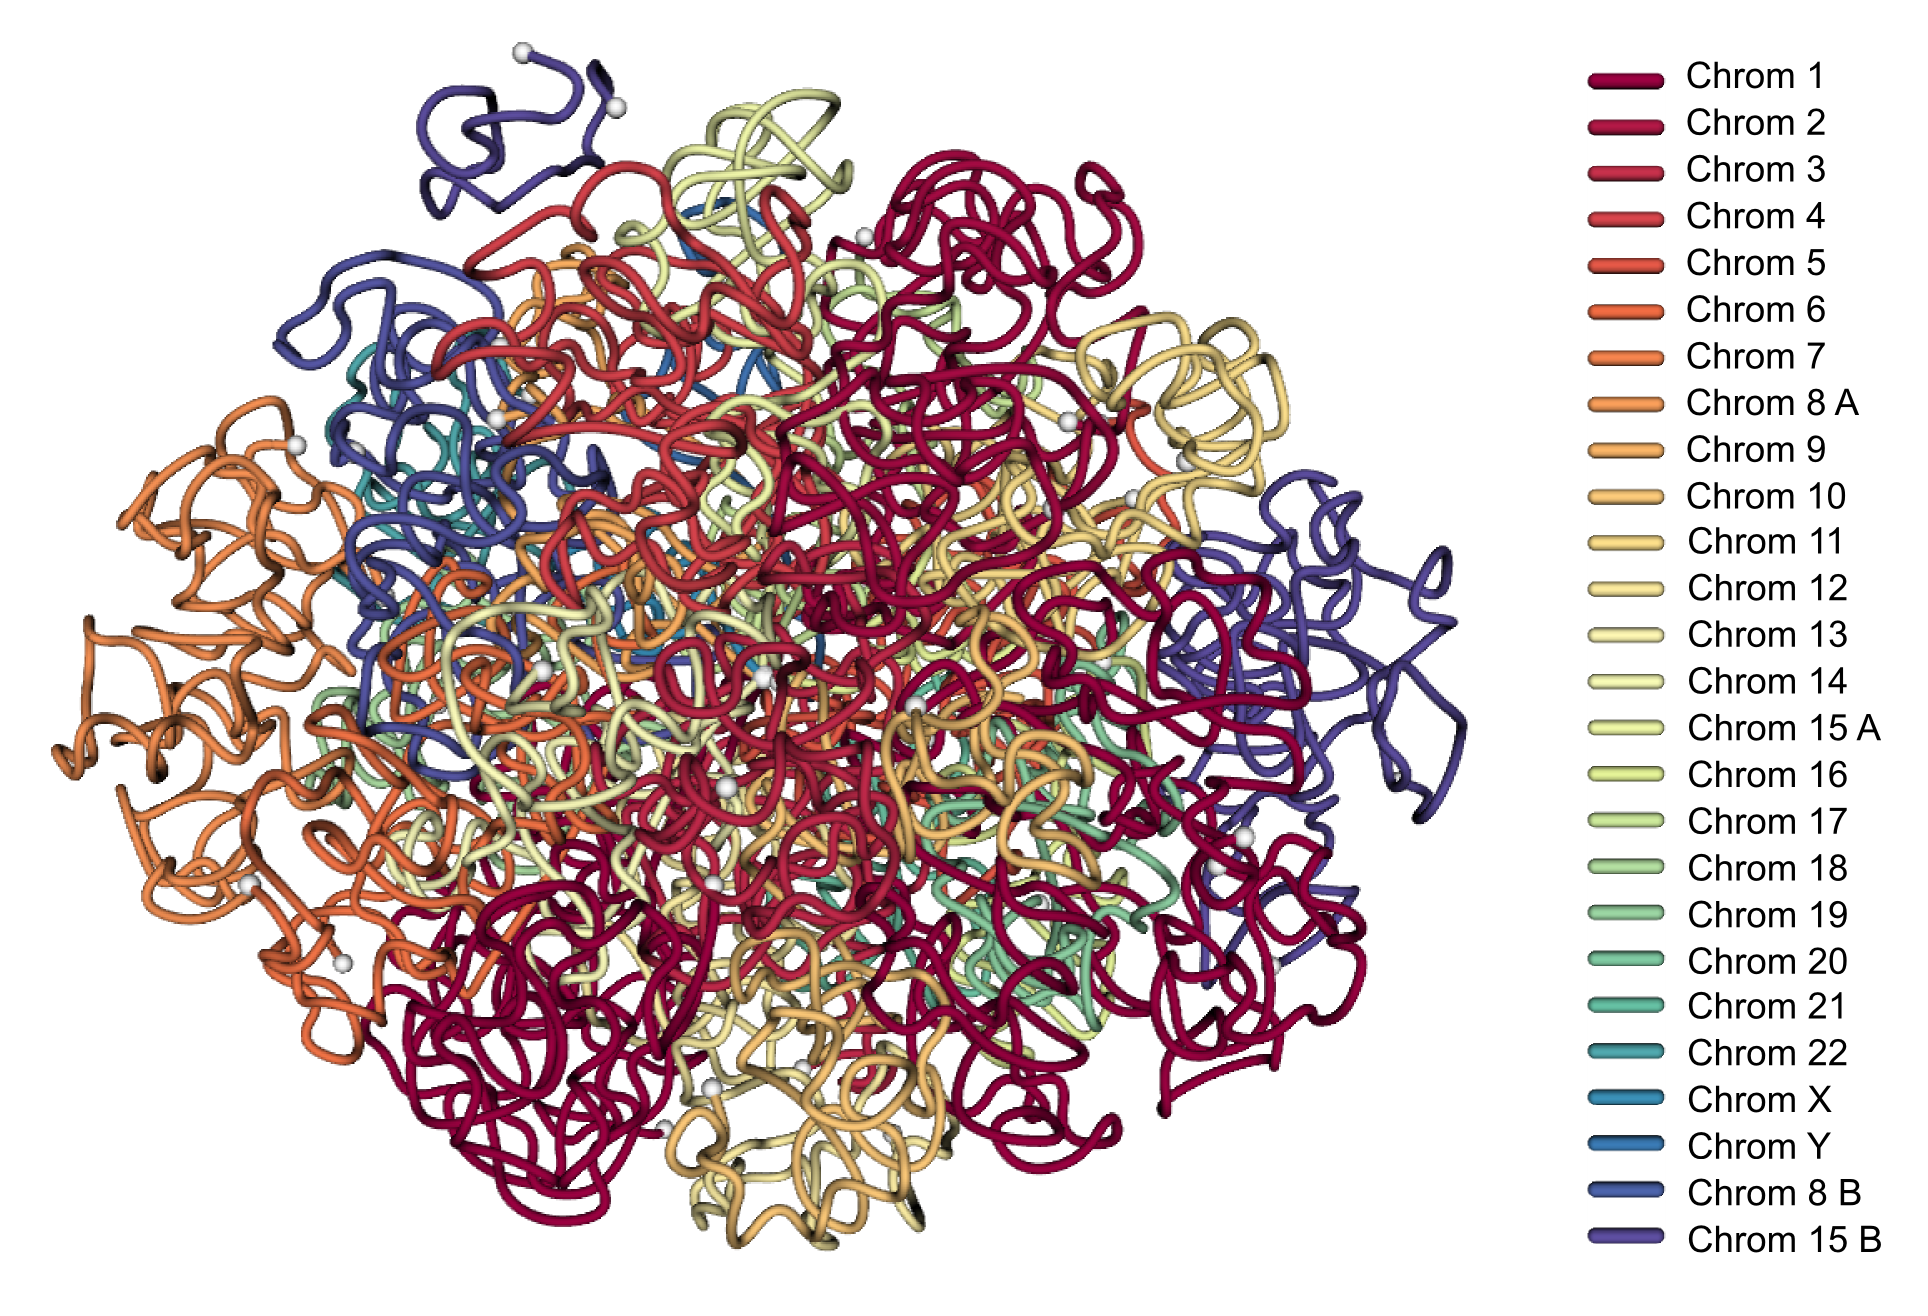
\includegraphics[width=0.6\textwidth]{\detokenize{figs/Nelle-3D/all_with_legend.png}}}
  \vspace{0.05\textwidth} \newline
  \subfloat[Chromosomes 1, 2, 3, 4 and 5]{\label{fig:3Dp3}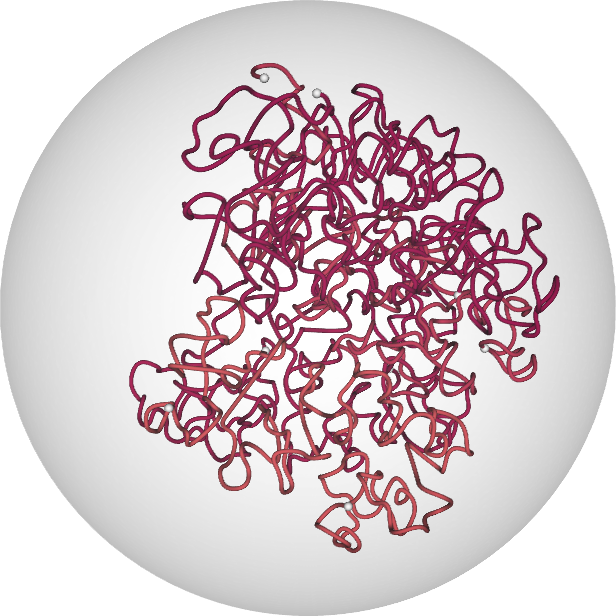
\includegraphics[width=0.3\textwidth]{\detokenize{figs/Nelle-3D/partial_3.png}}} \hspace{0.02\textwidth}
  \subfloat[Chromosomes 16, 17, 19, 20, 21, and 22]{\label{fig:3Dp1}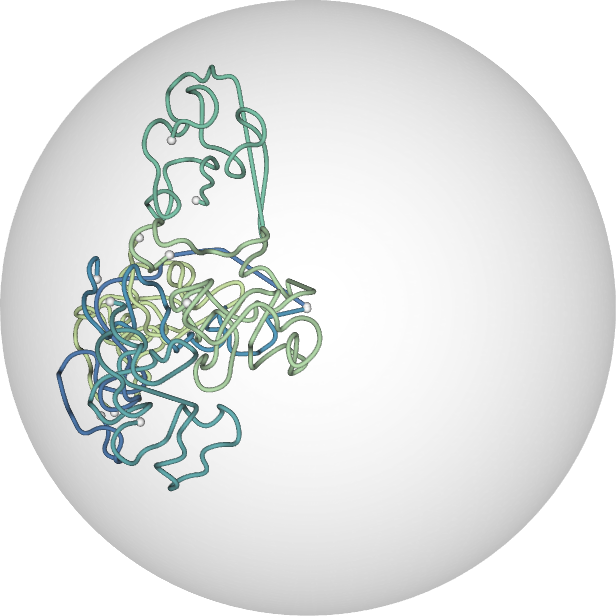
\includegraphics[width=0.3\textwidth]{\detokenize{figs/Nelle-3D/partial_1.png}}}
  \hspace{0.02\textwidth}
  \subfloat[Chromosomes 1, 2, 20 and 21]{\label{fig:3Dp4}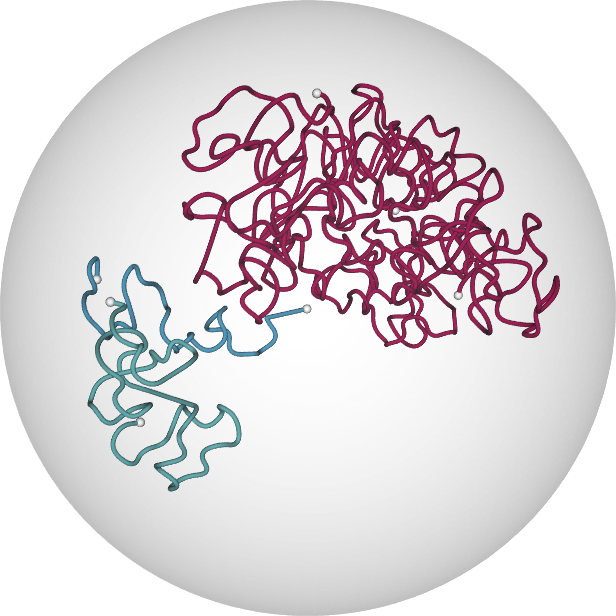
\includegraphics[width=0.3\textwidth]{\detokenize{figs/Nelle-3D/partial_4.png}}}
\caption{
\textbf{Three-dimensional modeling of KBM7 genome architecture}
 {\bf(a)} Three-dimensional structure of the 2~Mb region of chromosome 11 (chr11:1,000,000-3,000,000)
 which is centered around \emph{IGF2-H19} imprinting control region. This structure
 is inferred from normalized contact counts of KBM7-TM3C-1 data at 40~kb resolution
 using the Poisson model from \citet{varoquaux:statistical}.
 {\bf(b)} Three-dimensional structure of the KBM7 genome, which is haploid for all
chromosomes other than diploid chromosome 8 (8A, 8B) and partially diploid
chromosome 15 (15A, 15B) (see Methods for details of the 3D inference). Different
colors represent different chromosomes, and white balls represent chromosome ends.
 Same 3D structure as {\bf(b)} when confined to
 {\bf(c)} only a subset of long chromosomes,
 {\bf(d)} only a subset of small chromosomes,
 {\bf(e)} two small and two large chromosomes.
}
\label{fig:3D}
\end{figure}


Finally, to visualize the genome architecture of near-haploid KBM7 cells, we generated
a set of 3D structures using an optimization framework that alternates between inferring
the 3D configuration of beads that best summarize TM3C contacts~\citep{varoquaux:statistical}
and re-estimating the distribution of contact counts between diploid chromosomes.
Since this optimization is non-convex, we ran the optimization 1000 times and
selected the 100 structures with the highest log likelihoods (Methods).
Figure~\ref{fig:3D}b--e
plots the structure with highest likelihood inferred at 1~Mb resolution. Visual observation of
Figure~\ref{fig:3D}b suggests that individual chromosomes preserve their
territories in 3D (see also Additional File 3). In order to better visualize which chromosomes are closer
to each other, we plot subsets of different chromosomes in Figures~\ref{fig:3D}c--e.
Consistent with previous models~\citep{lieberman-aiden:comprehensive} and our
contact count heatmaps, we observe strong colocalization among the small gene-rich
chromosomes (16, 17, 19, 20, 21 and 22). However, chromosome 18, which is small but
gene-poor, does not colocalize with gene-rich small chromosomes in 3D
(Figure~\ref{fig:3D}c, Supplementary Fig.~\ref{suppfig:chr18in3D}).
We also observe colocalization of large chromosomes with each other, but not as
strongly as small chromosomes (Figure~\ref{fig:3D}d).
Visualization of two large and two small chromosomes clearly demonstrates
that the two sets of chromosomes are far from each other in our 3D models
(Figure~\ref{fig:3D}e).

%%%%% Results End %%%%%
%%%%%%%%%%%%%%%%%%%%%%

\section*{Discussion}
Catalyzed by the availability of genome-wide chromatin architecture data
generated using chromatin conformation capture assays, the field of regulatory
genomics has recently witnessed increased interest in the functional role of higher order DNA structure.
Organizational principles of eukaryotic nuclei that are uncovered by these
genome wide assays range from large scale patterns such as open/closed chromatin
compartments~\citep{lieberman-aiden:comprehensive} and topological
domains~\citep{dixon:topological} to more local patterns such as
silencing or activating of individual genes by altering the 3D proximity of enhancers
to gene promoters~\citep{ferraiuolo:three-dimensional, li:extensive}.
However, one important question that remains to be answered is how the
simultaneous proximity of more than two loci in the nucleus impacts gene
regulation. Current conformation capture assays cannot address this
question because they only characterize pairwise contacts that involve exactly two loci.

Here we demonstrated how to discover simultaneous multi-locus contacts using
a straightforward
conformation capture assay. We aimed at distinguishing between proximity
of multiple loci measured from different nuclei in the form of pairwise
contacts and simultaneous proximity between these loci within a single
nucleus. We showed that our TM3C assay, which can employ more than one
restriction enzyme at a time to increase chromatin digestion, results in
chimeras even within a single end of a short paired-end read. Accordingly, we developed
a two-phase  mapping pipeline that uses cleavage information to
extract from these chimeras informative contacts that involve two, three
or four loci. An additional advantage of TM3C is that it is significantly
simpler and yet provides increased resolution for the resulting contact
maps compared to current Hi-C assays.

It is important to note, however, that there are two drawbacks to
our assay compared to traditional Hi-C or TCC assays. The first drawback
is a tradeoff between resolution and the noise level of the data. Frequent
digestion of chromatin with multiple 4-cutters increases the resolution
but also the noise level of the data, as measured by the ratio between
inter and intrachromosomal reads (Additional file 2). The second drawback is
a tradeoff between the simplicity of the assay and the proportion of
informative reads from the paired-end sequencing. In the TM3C assay we omit
the steps of RE overhang biotinylation and streptavidin pull-down which
are present in both the Hi-C and TCC assays. This omission results in a
higher percentage of sonication products (non-informative read pairs)
in the sequencing libraries of TM3C (Additional file 2) which we
discard after read mapping.

Despite these drawbacks, we believe that TM3C is an effective
assay in profiling genome architecture---evident by the consistency
of our results with characteristic features of genome organization---with the
added benefit of revealing multi-locus contacts. In order to
demonstrate the utility of TM3C, we applied it to two human cell lines.
We specifically chose one of these cell lines as the near-haploid KBM7
which has been used in settings where having multiple copies of a
chromosome is problematic, such as loss-of-function genetic
screens~\citep{carette:haploid,burckstummer:reversible}. We first established that TM3C
contact maps are consistent with karyotypic features of KBM7 and
that KBM7 cells share common large scale organization with other
mammalian cell lines previously assayed by Hi-C. Focusing on
a well-studied locus (\emph{IGF2-H19}) that has been shown to be involved
in parent of origin specific long-range chromatin loops, we showed
that TM3C identifies multi-locus contacts (triples), more than half
of which were validated using PCR. Confirmed triples
involved intrachromosomal loops bringing together regions that
are more than megabases away in genomic distance as well as regions
from different chromosomes. Together with results from previous
FISH experiments that reveal \emph{IGF2} is located outside of
its chromosome territory in the majority of nuclei~\citep{mahy:gene},
our findings suggest that complex regulation of \emph{IGF2} and
\emph{H19} may involve interactions with multiple distal regions
simultaneously.

Another important aspect of our work is the modeling of 3D
organization of a human cell line without averaging data from
multiple copies of a chromosome or resolving the haplotype.
To date 3D modeling efforts on the human genome have been limited to
haploid chromosomes such as the X chromosome in male
cells~\citep{nagano:single-cell}, one chromosome or one portion of a
chromosome at a time~\citep{nagano:single-cell, bau:three-dimensional}
or have assumed artificially that only one copy of each chromosome
exists per cell~\citep{zhang:inference}.
In this work the near-haploid karyotype of KBM7 allowed us to
overcome these limitations
to infer whole-genome 3D models. By extending an algorithm that we developed
previously for haploid genomes~\citep{varoquaux:statistical} to handle the diploid
portions of KBM7 cells, we generated 3D models for this leukemia
cell line. Due to the lack of independent data available on KBM7 cells, we were unable
to verify our 3D models further or correlate them with features such
as histone modifications and transcription binding. However, our models
are consistent at the large scale with previous observations that
suggest chromosomes with similar sizes tend to be closer to each
other in 3D. It is also important to note that, similar to many previous approaches,
our 3D models are consensus structures that summarize the genome architecture of a
cell population. Capturing the heterogeneity of genome architecture across cells may be
possible in the future, especially in conjunction with single-cell techniques~\citep{nagano:single-cell}.

Overall, we showed that TM3C provides a framework to identify multi-locus
contacts genome-wide in conjunction with commonly used next generation sequencing
platforms that produce short paired-end reads (e.g., 100~bp Illumina).
We believe that with broader use of longer reads (e.g., Pacific Biosciences)
TM3C will be able to profile a larger number of multi-locus contacts
with higher signal-to-noise ratio. Such profiling is important in
understanding better the combinatorial regulation of gene expression
and complex chromatin loops that involve more than
two loci simultaneously.

\section*{Conclusion}

TM3C is a simple protocol for ascertaining genome architecture and can
be used to identify simultaneous contacts among three or four
loci. Application of TM3C to a near-haploid human cell line revealed
large-scale features of chromosomal organization and multi-way
chromatin contacts that preferentially link regions of open chromatin.

\section*{Materials and methods}
\subsection*{TM3C library generation}
Approximately six million NHEK and ten million KBM7 cells were fixed in 1.5\% formaldehyde at
room temperature for 10 minutes. The fixed cells were washed with TN buffer (10 mM Tris, 40
mM NaCl, pH 7.5) and collected by centrifugation at 600 g for 3 minutes. To
increase digestion efficiency, fixed cells (6 or 10 million / 122 ul) were
treated with SDS (add 3.8 ul of 10\% SDS to a final of 0.30\% SDS) at
64$^{\circ}\mathrm{C}$ for 10 minutes and then at 37$^{\circ}\mathrm{C}$
overnight (15 hours). The SDS concentration was reduced gradually to 0.10\% by
adding five times of 50 ul (1 x DpnII digestion buffer or NEB buffer 4 for
multiple enzymes) with mixing. Triton X-100 (38 ul of 20\% Triton X) was added
to 1.8\% concentration and the sample was incubated at 37$^{\circ}\mathrm{C}$
for 1 hour. Sample volume was adjusted to 600 ul by adding 1 X restriction
buffer, ATP (0.2 mM final) and BSA (100 ug/ml final). Digestion with
appropriate restriction enzymes (300 units each) was carried out on a rotate
shaker at 37$^{\circ}\mathrm{C}$ for 15 hours. We used high concentration NEB
enzymes to keep the final volume of the enzyme mixture less than 60 ul (1/10
reaction volume).

The digested samples were deactivated at 65$^{\circ}\mathrm{C}$ for 15 minutes
and then centrifuged at 15,000 g for 5 min. We recovered $\sim$95\% of cellular
DNA in the pellet fraction. The pellet fraction was re-suspended with T4
ligation buffer (15 ul 10 x buffer, 65 ul total) heated at
65$^{\circ}\mathrm{C}$ and mixed with 100 ul of melted 2.5\% low-melting
agarose.  We used 200 ul pipette to deliver the hot agarose sample to ice-cold
ligation buffer (800 ul of 1 x ligation buffer containing T4 ligase (4000
units, NEB) in a steady fashion within $\sim$5 seconds, on melted ice. Strings
of gel bead appeared instantly at 0$^{\circ}\mathrm{C}$. We sealed the tube
with parafilm and perform ligation at RT (23$^{\circ}\mathrm{C}$.) overnight on
top of a shaker ($\sim$300 rpm), then transfer the tube to a iced water bath.

The sample pellet was recovered by centrifugation at 20,000 g for 2 minutes,
then 10 ul of 1\% SDS (0.05\% final) was added and heated at
80$^{\circ}\mathrm{C}$ for 1 hour. Cross-links were reversed by treatment with
Proteinase K (200 ug/ml) at 65$^{\circ}\mathrm{C}$ and 300 rpm overnight (12
hours). Melted TM3C-agarose sample was incubated with RNase A (10 ug / 210 ul)
at 55$^{\circ}\mathrm{C}$ for 15 minutes and then purified by QIAquick gel
extraction protocol (QUIAGEN Inc., CA). Purified TM3C DNA was quantified using
both a NanoDrop spectrophotometer (Thermo Scientific) and a Qubit 2.0
Fluorometer. The Qubit quantification represents the more accurate DNA
concentration.

\subsection*{First phase mapping of sequence data}
We mapped the paired-end reads to the human reference genome (hg19) using the
short read alignment mode of BWA (v0.5.9) with default parameter settings. Each
end of the paired reads was mapped individually. We post-processed the
alignment results to extract the reads that satisfy the following three
criteria: (i) mapped uniquely to one location in the reference genome, (ii)
mapped with an alignment quality score of at least 30, (iii) mapped with an
edit distance of at most 3. Reads that satisfy these criteria are named
\emph{fully-mapped} (\textbf{F}), and the rest of the mapped reads that did not
satisfy these criteria are discarded from further analysis. We identified pairs
of fully-mapped reads that share a common identifier to generate the set of
contacts that we denote as \textbf{F-F} (fully-mapped - fully-mapped). The
reads that did not map to any location in this phase of mapping are named
\emph{non-mapped} and are analyzed further.

\subsection*{Second phase mapping of non-mapped reads}
Re-mapping the reads that are deemed \emph{non-mapped} in the initial mapping
is necessary to avoid discarding a significant number of informative reads for
an assay such as TM3C that uses a frequently cutting restriction enzyme (or
enzymes) for digestion. Due to the high frequency of cleavage sites in the
genome, TM3C is highly likely to capture ligations between DNA fragments from two
different loci in a single end of a read. We call each such read
\emph{chimeric} because the sequences do not come from a continuous piece of
DNA but instead from two loci that are in proximity in the three-dimensional
space. Therefore, for these chimeric ends, after splitting into smaller
fragments from the cleavage sites of the restriction enzymes used in the digestion
step, we applied a second phase of mapping.

Within each non-mapped read, we first counted the number of cleavage sites,
taking into account all the restriction enzymes that are used in the digestion
step for that specific library. We discarded
reads that contain more than two cleavage sites.
We also discarded reads that contain no cleavage sites because such reads
surely are not chimeric. We split the remaining reads that contain only one
cleavage site into two smaller fragments, preserving the entire cleavage
site on both adjacent fragments.
We mapped the two resulting fragments to the genome
using BWA with default parameter settings. The 3-point filtering criteria
mentioned in the previous section are applied to the aligned reads, but
allowing an edit distance of at most 1 to make sure we only extract the unique
and high quality mappings. The reads that are extracted from this phase of
mapping are named \emph{partially-mapped }(\textbf{P}) because they did not map
as a whole, but their constituent fragments were successfully mapped to
different loci. The two classes of
mapped reads (fully-mapped (\textbf{F}) and partially-mapped (\textbf{P}))
yield three possible types of contacts, namely \textbf{F}-\textbf{F},
\textbf{F}-\textbf{P} and \textbf{P}-\textbf{P}. The first set (F-F) is
extracted after the initial mapping in which each paired-end read can
contribute at most one interaction between two loci.
The second set (P-F) consists of paired-end reads with one end fully mapped and
the other end having either one or two smaller fragments that mapped to the
genome. If the latter contains only one mapped fragment, then the only
interaction is between this fragment and the fully-mapped end. However, if the
end has two mapped fragments, then this paired-end read produces three
contacts: one between the two mapped fragments on the partially-mapped end and
two others that have one side from a fragment from the partially-mapped end and
the other side from the fully-mapped end. In addition, the same paired-end read
produces one triple (i.e., interaction among three loci) of type P-F.
For the contacts of the third type (P-P), each paired-end can produce either
one, three or six pairwise contacts, depending on whether one or two fragments
from each end are successfully mapped. If only one fragment from one end and
two from the other is mapped, then, similar to the case of P-F, three pairwise
contacts and one triple is produced.
If both ends have two mapped fragments, then six pairwise contacts, four triples
(of type P-P) and one quadruple (i.e., contact among four loci) are produced.

\subsection*{Normalization of contact maps}

For each possible pair of 1~Mb loci, we refer to the total number of read
pairs that link the two loci as the {\em contact count}, and we refer to the
two-dimensional matrix containing these contact counts as the {\em raw contact
map}. To normalize the $3113 \times 3113$ raw contact maps, we extended the
iterative correction procedure, ICE~\citep{imakaev:iterative}, for a nearly
haploid genome. First, we corrected for the bias caused by the partial
diploidy of the genome. For that, we constructed a ``deduplicated'' contact
counts matrix, where contact counts associated with diploid loci are divided
into two equal parts, each of which is associated with one of the
homologous chromosomes. Contact counts between two different copies of diploid
chromosomes/regions are set to 0. The deduplicated matrix is akin to
an artificially created allele-specific contact counts matrix, where
homologous chromosomes interact in identical ways and do not interact with
each other. As a preprocessing step, we ranked loci by their percentage of
intrachromosomal contacts with zero counts and filter out the top 10\% of this
list. This filtering removes all loci for which the signal to noise ratio is
too low (typically, regions of low mappability). Last, we applied ICE, a
method that attempts to eliminate systematic biases in Hi-C data. ICE
assumes that the bias for each entry can be decomposed as the product of the biases
associated with each locus, and estimates a bias vector $\beta$ under the equal
visibility hypothesis: the coverage of counts should be uniform. The tensor
product $\beta \otimes \beta$ generates a bias matrix that can be used to
convert the raw contact map into a normalized contact map. To generate a
contact count matrix of the original size, we summed all counts from
homologous chromosomes associated with the same loci. This procedure
yields a ($3113 \times 3113$) contact counts matrix for which diploid
loci interact twice as much as haploid loci.

\subsection*{Eigenvalue decomposition}
We carried out eigenvalue decomposition on the normalized contact maps of KBM7
and NHEK TM3C datasets as described in \citet{lieberman-aiden:comprehensive}.
For each chromosome we used the intrachromosomal contact matrices at 1 Mb
resolution. We calculated the Pearson correlation between each pair of rows
of the contact matrix and apply eigenvalue decomposition
(using the eig function in MATLAB) to the correlation matrix.
The sign of either the first or the second eigenvector defines chromosome
compartments for each chromosome. Similar to \citet{lieberman-aiden:comprehensive},
we used the second eigenvector in cases where the first eigenvector values are
either all positive or all negative. To map signs of eigenvectors to open/closed
compartment labels we used GC content as a marker. For each chromosome the sign
with higher GC content is selected as open chromatin. We then compared the
percentage of 1~Mb bins that are assigned the same compartment label by TM3C data
versus previously published Hi-C data in four human cell lines
(H1-hESC, IMR90~\citep{dixon:topological};  K562, GM06990~\citep{lieberman-aiden:comprehensive}).


\subsection*{Topological domain analysis}
We identified topological domains using a previously described hidden Markov
model-based software tool~\citep{dixon:topological}. To facilitate direct
comparison with the previously published topological domains in human cell
lines, we carried out the domain calling for these published datasets using
the human GRCh36/hg19 assembly. We applied the topological domain calling on
normalized contact maps of our TM3C data at 40 kb resolution.
To measure the consistency between the topological domains inferred from
TM3C and those from published Hi-C data, we calculated the overlap of domain
boundaries obtained between these two assays. We deemed two boundaries, one
from each assay, as overlapping if they overlap by at least 1~bp or are
adjacent to each other, as described in~\citet{dixon:topological}.

\subsection*{Contacts among regions with the same compartment label}
We used compartment labels assigned by the eigenvalue decomposition as described
above and computed the number of read pairs that define double and triple contacts
between two or among three regions all with the same compartment label
(all open or all closed) or at least two with opposite labels (mixed). We used
only interchromosomal doubles and interchromosomal triples (linking three different chromosomes)
for this analysis and eliminated regions that have less than 50\% uniquely mappable bases.
We then computed the number of all possible pairs and triples
of 1~Mb windows and segregated this number into three groups (all open, all closed, mixed)
giving us the expected percentages of contacts that should fall into each group.
With exactly equal numbers of open and closed compartments for each chromosome,
these percentages would be 25\%, 25\%, 50\% for pairs of compartments and
12.5\%, 12.5\%, 75\%  for triples of compartments for the groups of all open,
all closed and mixed, respectively. We then reported the ratio between the percentage
of observed double and triple contacts to expected percentages within each of these
three groups. A ratio $>$1 represents an enrichment for the observed
contacts for that compartment label group.

\subsection*{Contacts among regions with similar numbers of DHSs}
We performed an analysis similar to the compartment label analysis described above
using joint (UW--Duke) DNase hypersensitivity peak calls for the six Tier 1 cell lines
(GM12878, H1-hESC, HeLa-S3, HepG2, HUVEC, K562)
downloaded from \url{http://ftp.ebi.ac.uk/pub/databases/ensembl/encode/integration_data_jan2011/byDataType/openchrom/jan2011/fdrPeaks}.
Since there is no DNase data for KBM7 we reported results for only K562
which is also a leukemia cell line. We computed for each 1~Mb window with
mappability of at least 50\% the number of DHS peaks that overlap with this
window. We sorted all these windows by decreasing number of DHSs
and labeled the top 50\% as ``high'' and bottom 50\% as ``low'' DNase
sensitivity. We then calculated and reported the expected over observed
percentage of doubles and triples as described for compartment labels.

\subsection*{Contacts within the same topological domain}
After carrying out the topological domain calling using our KBM7-TM3C-1 data,
we computed the percentage of intrachromosomal doubles and triples that
link loci within the same topological domain.
To estimate the significance of the observed percentages, we randomly
shuffled topological domains by preserving the distribution of
the domain lengths for each chromosome arm as described in
 \citet{ay:statistical}. We reported the mean and the standard deviation
for the percentage of within domain doubles and triples across 100
randomized shufflings.


%\subsection*{Contacts among regions annotated as enhancers and promoters}
%For the six Tier 1 ENCODE cell lines we downloaded the annotation labels assigned
%using two different semi-automated genomic annotation tools from \url{http://ftp.ebi.ac.uk/pub/databases/ensembl/encode/integration_data_jan2011/byDataType/segmentations/jan2011/Combined_7_state}.
%Out of seven annotation labels we extracted the regions with labels
%``E: Predicted enhancer'' and ``TSS: Predicted promoter region including
%transcription start site'' which we refer to as enhancer and promoter,
%respectively. For each 40~kb region in the genome, which is the highest
%resolution at which we analyze KBM7 contact maps, we determined whether
%it overlaps with at least one enhancer and one promoter (EP), one or more
%enhancers but no promoter (E), one or more promoters but no enhancers (P)
%or no promoter and no enhancer (N). Using these four new labels, we computed
%the percentages of all 64 possible label combinations for the set of all
%triples from the KBM7-TM3C-1 library. We then reported the percentage of
%triples that link two windows with label P and one window with label N
%(one P-P) and that link three windows all with label P (multi P-P).
%For enhancer-promoter contacts, we reported the percentage of triples
%with one window labeled as E or EP, one window labeled as P or EP and
%one window labeled as N (one E-P) and the percentage with all windows
%labeled as E, P or EP excluding the case of all Ps or all Es (multi E-P).
%
%To assess the significance of the four percentages described above, we
%randomly shuffled the windows linked by each triple 100 times and compute
%the same percentages for this ensemble of shuffled triples. For
%interchromosomal triples this shuffling is as straightforward as picking
%three random windows on three different chromosomes. For intrachromosomal
%or mixed triples we shuffle only by shifting the genomic coordinates of
%each locus by a random amount to preserve the genomic distances between
%loci that are on the same chromosome to avoid biases due to higher
%contact frequency between regions separated by a smaller genomic distance.
%We then reported for each group (one P-P, multi P-P, one E-P, multi E-P)
%the ratio of observed percentages from actual triples to the percentages
%computed from shuffled triples.


\subsection*{Inference of the 3D structure}

We modeled each chromosome as a series of beads on a string, spaced
approximately 1~Mb apart. We denote by $\textbf{X} = (x_1,\ldots,x_n) \in
\mathbb{R}^{3 \times n}$ the coordinate matrix of the structure, where $n$
denotes the total number of beads in the genome including the newly introduced
chromosomes 8B and 15B ($n=3289$ for the KBM7 genome), and $x_i\in \mathbb{R}^3$ represents the 3D
coordinates of the $i$-th bead. Contacts from TM3C data can be summarized as
an $m \times m$ matrix $\textbf{c}$, where each entry $c_{kl}$ corresponds to
the observed contact count between loci $k$ and $l$. Because contact information
does not distinguish between homologous chromosomes, $m$ only includes one
copy of each chromosome and $m<n$. For loci in diploid regions, the contact counts are the sum of contact counts due to each copy of the region. If we denote by $\Phi:[1,n]\rightarrow [1,m]$ the mapping that associates a bead $i$ to a locus $\Phi(i)$ of the contact count matrix, this means that the contact count $c_{kl}$ between loci $k$ and $l$ is the sum of counts due to interactions between beads in $\Phi^{-1}(k)$ and $\Phi^{-1}(l)$. For any two beads $i$ and $j$ mapping respectively to loci $k=\Phi(i)$ and $l=\Phi(j)$, let us denote by $0\leq \mu_{ij}\leq 1$ the proportion of counts in $c_{kl}$ due to interactions between beads $i$ and $j$. Since all contact counts must be accounted for by interactions between beads, we must have for any loci $k$ and $l$:
$$
\sum_{i\in\Phi^{-1}(k)\,,j\in\Phi^{-1}(l)} \mu_{ij}=1\,.
$$
We propose to jointly infer the structure $\mathbf{X}$ and the distributions of contact counts $\mu_{ij}$'s by maximizing the likelihood of the observed contact counts. For that purpose,
we modeled the contact frequencies $(\mu_{ij}c_{\Phi(i) \Phi(j)})_{(i,j) \in
\mathcal{D}}$ ($\mathcal{D}$ is the set of non-zero contact counts) as
independent Poisson random variables, where the Poisson parameter of $\mu_{ij}
c_{\Phi(i)\Phi(j)}$ is a decreasing function of the Euclidean distance
$d_{ij}(\textbf{X})$ between beads $i$ and $j$. Our and others' previous
work suggested that the relationship between $\mu_{ij}c_{\Phi(i)\Phi(j)}$ and $d_{ij}$
is approximately of the form $d_{ij}(\mathbf{X})^\alpha$, with $\alpha = -3$
\citep{lieberman-aiden:comprehensive,fudenberg:higher-order,varoquaux:statistical}.
We can then express the likelihood of the model as:
\begin{equation}
\ell(\mathbf{X}, \mu) = \prod_{i, j} \frac{(d_{ij}^{\alpha})^{\mu_{ij}
c_{\Phi(i)\Phi(j)}}}
					   {(\mu_{ij} c_{\Phi(i)\Phi(j)})!}
		         \exp (- d_{ij}^{\alpha}) \,.
\end{equation}
To infer the position of each bead, we maximized the log likelihood of the
model which is:
\begin{equation}
\mathcal{L}(\mathbf{X}, \mu) = \sum_{i, j} \mu_{ij} c_{\Phi(i)\Phi(j)} \alpha \log(d_{ij})
- d_{ij}^{\alpha} - \log(\mu_{ij} c_{\Phi(i)\Phi(j)}!) \,.
\end{equation}
In practice, we solved the following relaxation since $\mu_{ij}c_{\Phi(i)\Phi(j)}$ may not
have integer values
\begin{equation}
\mathcal{L}(\mathbf{X}, \mu) = \sum_{i, j} \mu_{ij} c_{\Phi(i)\Phi(j)} \alpha \log(d_{ij})
- d_{ij}^{\alpha} - \log( \Gamma(\mu_{ij} c_{\Phi(i)\Phi(j)} + 1)) \,,
\end{equation}
with the following constraints:
\begin{itemize}
\item $d_{ij} \leq d_{max}$. To find a suitable $d_{max}$, we first computed
the expected distances $c_{i, i+1} ^{-1 / 3}$ for adjacent beads of haploid
chromosomes. We set $d_{max}$ to the 97\% quantile, thus excluding outliers
values arising in the normalization procedure.
\item $0.3 \leq \mu_{ij} \leq 0.7$, where $i$ and $j$ corresponds to loci from
the same copy of a diploid chromosomes.
\end{itemize}

To optimize this non-convex function, we iterated between two steps: (1) infer
the 3D structure $\mathbf{X}$; (2) re-estimate the distribution of contact counts $\mu_{ij}$ between
diploid chromosomes. The first step is solved using an interior point method,
as described in \citet{varoquaux:statistical}.
For the second step, the optimization problem can be performed with respect to
each pair of loci $k$ and $l$ independently. Thus we perform a grid search
on $\{\mu_{ij} | \Phi(i) = k, \Phi(j) = l\}$, with a step size of 0.01.

We ran the
optimization 1000 times varying the initialization of the distribution of the
contact counts, and another 1000 times varying the initial structure
$\textbf{X}$. We then selected the top 100 structures with the highest log
likelihoods.

\bigskip % END OF METHODS

%%%%%%%%%%%%%%%%%%%%%%%%%%%%%%%%
\section*{List of abbreviations used}
3C: chromatin conformation capture, TM3C:  tethered multiple 3C, TCC: tethered
3C, ICR: imprinting control region, PCR: polymerase chain reaction,
RE: restriction enzyme, Ph+: Philadelphia chromosome positive,
CpG: Cytosine---phosphate---Guanine, DHS: DNase hypersensitive site,
TSS: transcription start site.

\section*{Competing interests}
The authors declare that they have no competing interests.

\section*{Authors' contributions}
A.R.H., T.H.V. and W.S.N. conceived the project. T.H.V. developed the assay and
carried out the experiments. F.A. analyzed the data under the supervision of W.S.N.
N.V. inferred 3D structures under the supervision of J.V.  F.A.,  W.S.N., N. V. and
T.H.V. wrote the manuscript. All authors discussed and edited the manuscript.


\section*{Acknowledgements}
%  \ifthenelse{\boolean{publ}}{\small}{}
We are grateful to Zhi-jun Duan for helpful comments.
This work was financially supported by the National Institutes of Health
(grant R01 GM09031 to ARH and U41 HG007000 to WSN), a Computing Research Association CIFellows
award (NSF award CIF 1136996 to FA), the European Research Council
(grant SMAC-ERC-280032 to JPV/NV), the European Commission
(grant HEALTH-F5-2012-305626 to JPV/NV) and the French National
Research Agency (grant ANR-11-BINF-0001 to JPV/NV).
\lineskip=0pt

\section*{Tables}
 \subsection*{Table 1 - Summary of datasets generated in this paper.}
 \label{table:libs}
\par \mbox{}
\par\mbox{
%{\footnotesize
%\begin{tabular}{lccccccc}
\begin{tabular}{l|c|cccc|c}
\multirow{3}{*}{\textbf{Cell Type}}  & \multirow{3}{*}{\textbf{Tethering}} & \multicolumn{4}{|c|}{\textbf{Restriction Enzymes (REs)}}  & \multirow{3}{*}{\textbf{Identifier}} \\
&   & \textbf{AluI} & \textbf{MboI/DpnII}  & \textbf{MspI} & \textbf{NlaIII} & \\
&  & AG$|$CT & $|$GATC  & C$|$CGG & CATG$|$  & \\\hline\hline
%rows
NHEK  & Yes & & $\checkmark$ &  & & NHEK-TM3C-1   \\
KBM7 & Yes & & $\checkmark$ &  &  & KBM7-TM3C-1   \\
KBM7  & Yes & $\checkmark$ & $\checkmark$ & $\checkmark$  & $\checkmark$  & KBM7-TM3C-4  \\
KBM7 (gDNA) & No & $\checkmark$ & $\checkmark$ & $\checkmark$  & $\checkmark$  & KBM7-MCcont-4  \\
\end{tabular}
%}
}

{
 \subsection*{Table 2 - Summary of informative pairwise and multi-locus contacts for each KBM7 library.}
 \label{table:contacts}
\par \mbox{}
\par\mbox{
%{\footnotesize
%\begin{tabular}{lccccccc}
\begin{tabular}{l|c|c|c|c}
\textbf{Library} & \textbf{Total Reads} & \textbf{Doubles (pairwise)} & \textbf{~Triples~} & \textbf{Quadruples} \\\hline\hline
%\multirow{2}{*}{NHEK-TM3C-1} & \multirow{2}{*}{89,383,720} & 2,775,647 & 20,565 & 71 \\
%& & & & \\
& & & & \\
\multirow{5}{*}{KBM7-TM3C-1} & \multirow{5}{*}{95,000,000} & 14,830,477 & 211,249 & 1,676  \\
& & (15.61\%) & (0.22\%) & (0.002\%) \\
& & inter: 8,036,033 & inter: 92,959 &inter: 672\\
& & intra: 6,794,444 & intra: 28,930 &intra: 38\\
& & & mixed: 89,360 & mixed: 966\\\hline\hline
%
& & & & \\
\multirow{5}{*}{KBM7-TM3C-4} & \multirow{5}{*}{72,800,218} & 13,858,985 & 816,625 & 25,158  \\
& & (19.04\%) & (1.12\%) & (0.034\%) \\
& & inter: 11,544,137 & inter: 594,052 &inter: 15,889 \\
& & intra: 2,314,848 & intra: 22,787 &intra: 85\\
& & & mixed: 199,786& mixed: 9,184 \\
\end{tabular}
%}
}

 \subsection*{Table 3 - Summary of intrachromosomal read orientations for different contact types (KBM7-TM3C-1).}
 \label{table:orientation}
\par \mbox{}
\par\mbox{
\begin{tabular}{l|c|cccc}
\textbf{Contact Type} & \textbf{Genomic Dist.} & \multicolumn{4}{|c}{\textbf{Read Orientations (end1/end2)}}  \\\hline\hline
%
\multirow{5}{*}{Doubles (F-F)} & & \textbf{\texttt{~+/+~}} & \textbf{\texttt{~+/-~}} & \textbf{\texttt{~-/+~}} & \textbf{\texttt{~-/-~}}  \\\cline{3-6}
& \multirow{2}{*}{All} & \multirow{2}{*}{1.8\%} & \multirow{2}{*}{ 48.2\%} & \multirow{2}{*}{ 48.2\%} & \multirow{2}{*}{ 1.8\%} \\
& & & & & \\
& \multirow{2}{*}{$>$~1~kb} & \multirow{2}{*}{24.9\%} & \multirow{2}{*}{ 25.1\%} & \multirow{2}{*}{ 25.1\%} & \multirow{2}{*}{ 24.9\%} \\
& & & & & \\\hline\hline
\multirow{5}{*}{Triples (F-P)} & & \textbf{\texttt{~+/++,-/--~}}& \textbf{\texttt{~+/+-,-/-+~}} & \textbf{\texttt{~+/-+,-/+-~}} & \textbf{\texttt{~+/--,-/++~}} \\\cline{3-6}
& \multirow{2}{*}{All} & \multirow{2}{*}{0.1\%}  & \multirow{2}{*}{49.7\%} & \multirow{2}{*}{0.2\%} & \multirow{2}{*}{50\%} \\
& & & & & \\
& \multirow{2}{*}{$>$~1~kb} & \multirow{2}{*}{24.5\%} & \multirow{2}{*}{25.8\%} & \multirow{2}{*}{25.3\%} & \multirow{2}{*}{24.4\%}\\
& & & & & \\\hline\hline
\multirow{5}{*}{Triples (P-F)} & & \textbf{\texttt{~++/+,--/-~}} & \textbf{\texttt{~++/-,--/+~}} & \textbf{\texttt{~+-/+,-+/-~}} & \textbf{\texttt{~+-/-,-+/+~}} \\\cline{3-6}
& \multirow{2}{*}{All} & \multirow{2}{*}{0.2\%} & \multirow{2}{*}{49.9\%} & \multirow{2}{*}{49.7\%} & \multirow{2}{*}{0.2\%} \\
& & & & & \\
& \multirow{2}{*}{$>$~1~kb} & \multirow{2}{*}{25.6\%} & \multirow{2}{*}{24.1\%} & \multirow{2}{*}{25.4\%} & \multirow{2}{*}{25.0\%} \\
& & & & & \\
\end{tabular}
}
}

\section*{Supplementary Figures}
%\addcontentsline{toc}{section}{Supplementary Figures}

%\begin{enumerate}
%  \item 2D histogram bias plots before and after normalization for both KBM7 and NHEK libs
%  \item Normalized inter-chromosomal contact heatmaps for each of the four libs
%  \item Ploidy tracks for KBM7 and NHEK
%  \item PCR gel pictures that are not used in the main text
%  \item Figure with sonication fragments making a peak at selected length (can be dangerous to show this)
%\end{enumerate}

\begin{figure}[ht!]
\begin{center}
\includegraphics[width=0.6\textwidth]{suppfigs/cutSiteComparison.pdf}
\end{center}
\caption{Number of restriction enzyme cut sites across the human genome.}
{Histograms of the number of cut sites within 40~kb windows across the human
    genome for each digestion system. HindIII, the most commonly used RE
    for creating Hi-C libraries, recognizes a 6~bp cut site, whereas AluI,
    MboI, MspI and NlaIII all cleave from 4~bp cut sites. For TM3C-1 libraries
    only MboI was used. For TM3C-4 libraries all four 4~bp cutters were used
    together to digest crosslinked chromatin. The theoretical resolution that can
    be achieved by each digestion system is inversely proportional to the
    RE cut site frequency. The mean number of cut sites per 40~kb suggests that
    TM3C-1 (99.5) and TM3C-4 (501.7) can achieve around 9 and 43 times
    higher resolution compared to using HindIII (11.7).
}
\label{suppfig:cutSiteComparison}
\end{figure}
\clearpage

\begin{figure}
\begin{center}
  \subfloat[F-F]{
  \includegraphics[width=0.45\textwidth]{\detokenize{suppfigs/interchrHeatmaps/heatmaps-beforeNormalization/F-F/KBM7-100bp-TMC-1.pdf}}}
  \hspace{0.01\textwidth}
  \subfloat[P-F]{
  \includegraphics[width=0.45\textwidth]{\detokenize{suppfigs/interchrHeatmaps/heatmaps-beforeNormalization/P-F/KBM7-100bp-TMC-1.pdf}}}
  \newline
  \subfloat[P-P]{
  \includegraphics[width=0.45\textwidth]{\detokenize{suppfigs/interchrHeatmaps/heatmaps-beforeNormalization/P-P/KBM7-100bp-TMC-1.pdf}}}
  \hspace{0.01\textwidth}
  \subfloat[All]{
  \includegraphics[width=0.45\textwidth]{\detokenize{suppfigs/interchrHeatmaps/heatmaps-beforeNormalization/together/KBM7-100bp-TMC-1.pdf}}}
\end{center}
\caption{Chromosome contact maps of different contacts types for KBM7-TM3C-1.}
{Pairwise raw contact counts are averaged over all pairs of mappable
    1~Mb windows between the two chromosomes. Contacts that are of type
    (a) fully mapped/fully mapped (both ends mapped completely),
    (b) partially mapped/fully mapped (one end mapped completely and one end mapped after second phase of mapping)
    and (c) partially mapped/partially mapped (both ends mapped after second phase of mapping)
    are plotted separately. For (d) we aggregated all these three types of contacts.
}
\label{suppfig:compareThreeTypes}
\end{figure}
\clearpage


\begin{figure}
\begin{center}
\includegraphics[width=0.8\textwidth]{figs/KBM7anomalies/KBM7-diploidRegions-cropped.pdf}
\end{center}
\caption{Ploidy track for select chromosomes from KBM7 TM3C data.}
{Plot of total contact count from each 1 Mb region to all other regions
 (both intra and interchromosomal) in the genome for a haploid (chr. 4),
 a diploid (chr. 8) and a partially diploid (chr. 15) chromosome. The diploid
 region of chromosome 15 is approximately 29 Mb (61--90 Mb).}
 \label{suppfig:KBM7ploidyTrack}
\end{figure}
\clearpage

\begin{figure}
\begin{center}
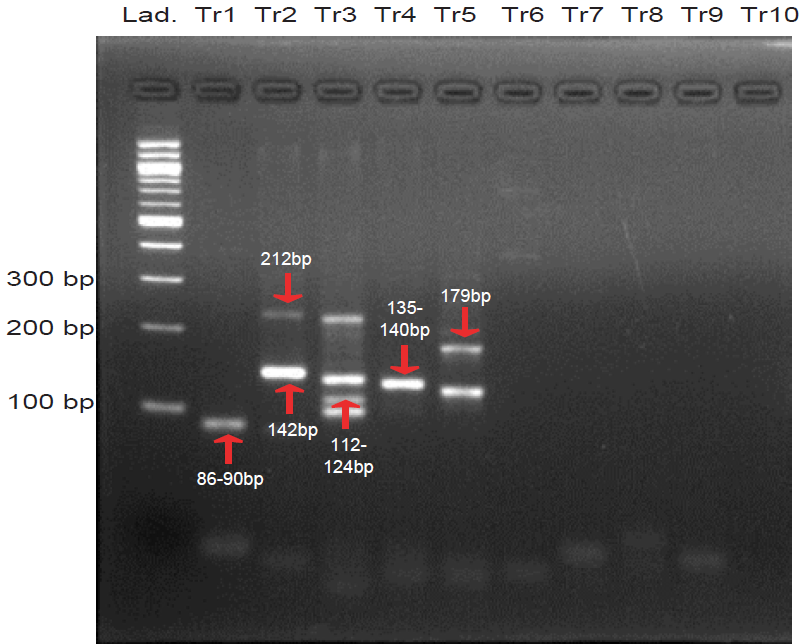
\includegraphics[width=0.9\textwidth]{suppfigs/tenTriples.png}
\end{center}
\caption{PCR verification of triples 1--10 listed in Main Figure~5.}
{Lanes are: 100~bp ladder, triples 1 to 10. For each experiment all
    three primers (e.g., 1a+1b+1c) designed for that triple are used
    simultaneously. Expected product sizes for each triple are listed
    in Supplementary Table~\ref{supptable:PCRprimers} and corresponding 
    PCR products with approximate sizes are indicated by red arrows.
    Triples 1--5 showed PCR products in this gel, and triple 6 showed
    one product in another gel (Supplementary Fig.~\ref{suppfig:only5and6Gels}).
}
\label{suppfig:tenTriples}
\end{figure}
\clearpage


\begin{figure}
  \begin{center}
  \subfloat[Triple 5 only]{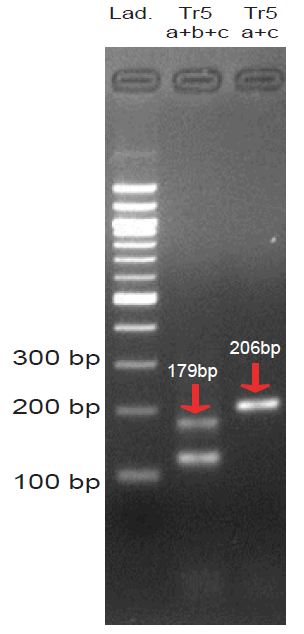
\includegraphics[width=0.277\textwidth]{\detokenize{suppfigs/triple5onlyGel.png}}}
  \hspace{0.02\textwidth}
  \subfloat[Triple 6 only]{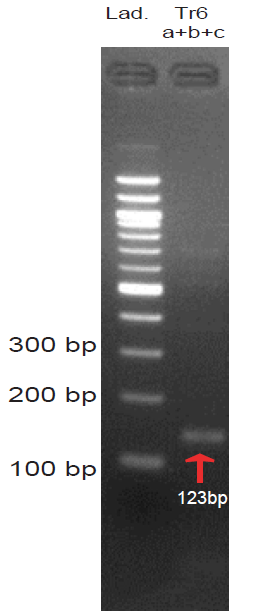
\includegraphics[width=0.2\textwidth]{\detokenize{suppfigs/triple6onlyGel.png}}}
  \end{center}
\caption{Additional PCR experiments for triples 5 and 6.}
    {(a) Triple 5 PCR gel. Lanes are: 100~bp ladder, 5a+5b+5c primers and only 5a+5c primers.
    (b) Triple 6 PCR gel. Lanes are: 100~bp ladder and 6a+6b+6c primers. 
    Expected product sizes for each case are listed in Supplementary 
    Table~\ref{supptable:PCRprimers} and corresponding
    PCR products with approximate sizes are indicated by red arrows.}
\label{suppfig:only5and6Gels}
\end{figure}
\clearpage


\begin{figure}
\begin{center}
  \subfloat[Triple~1--end~1]{
  \includegraphics[width=1\textwidth]{suppfigs/triple1-end1.pdf}}
  \hspace{0.01\textwidth}
  \subfloat[Triple~1--end~3]{
  \includegraphics[width=1\textwidth]{suppfigs/triple1-end3.pdf}}
\end{center}
\caption{Methylation status of the distal contact partners of \emph{IGF2-H19} ICR for triple 1.}
{UCSC genome browser snapshots of the tracks that display the methylation
    status of CpG dinucleotides in six ENCODE cell types for the two loci
    that are distal contact partners of ICR in triple 1. Methylation scores
    are color coded with orange for ``methylated'', purple for ``partially methylated''
    and blue for ``unmethylated''. The figure displays a 20~kb region centered on
    (a) triple 1--end 1 located on chromosome 11, and
    (b) triple 1--end 3 located on chromosome 17.
    End 2 is located within 40~kb of the ICR.
}
\label{suppfig:triple1methyl}
\end{figure}
\clearpage

\begin{figure}
\begin{center}
  \subfloat[Triple~2--end~2]{
  \includegraphics[width=1\textwidth]{suppfigs/triple2-end2.pdf}}
  \hspace{0.01\textwidth}
  \subfloat[Triple~2--end~3]{
  \includegraphics[width=1\textwidth]{suppfigs/triple2-end3.pdf}}
\end{center}
\caption{Methylation status of the distal contact partners of \emph{IGF2-H19} ICR for triple 2.}
{Similar snapshots as Supplementary Fig.~\ref{suppfig:triple1methyl} above for 20~kb
    region centered on (a) triple 2--end 2 located on chromosome 11, and
    (b) triple 2--end 3 located on chromosome 8.
    End 1 is located within 40~kb of the ICR.
}
\label{suppfig:triple2methyl}
\end{figure}
\clearpage

\begin{figure}
\begin{center}
  \subfloat[Triple~3--end~1]{
  \includegraphics[width=1\textwidth]{suppfigs/triple3-end1.pdf}}
  \hspace{0.01\textwidth}
  \subfloat[Triple~4--end~3]{
  \includegraphics[width=1\textwidth]{suppfigs/triple4-end3.pdf}}
\end{center}
\caption{Methylation status of the distal contact partners of \emph{IGF2-H19} ICR for triples 3 and 4.}
{Similar snapshots as Supplementary Fig.~\ref{suppfig:triple1methyl} above for (a) 20~kb
    region centered on triple 3--end 1 located on chromosome 11, and
    (b) 40~kb region centered on triple 4--end 3 located on chromosome 4.
    Ends 2 and 3 for triple 3, and ends 1 and 2 for triple 4 are located within 40~kb of the ICR.
}
\label{suppfig:triple3methyl}
\end{figure}
\clearpage

\begin{figure}
 \begin{center}
  \includegraphics[width=1.0\textwidth]{suppfigs/IGF2expScreenshot.pdf}
 \end{center}
\caption{Gene expression measured by RNA-seq for the \emph{IGF2-H19} locus.}
{Snapshot of 200~kb region taken from the KBM7 genome browser (B\"{u}rckst\"{u}mmer et
    al.) that includes the \emph{IGF2} and
    \emph{H19} genes. RNA-seq measurements show that \emph{H19} is expressed,
    whereas \emph{IGF2} is not. This mode of \emph{IGF2-H19} expression is
    consistent with the maternal expression pattern of human chromosome 11.
}
\label{suppfig:IGF2expr}
\end{figure}
\clearpage

\begin{figure}
  \begin{center}
  \subfloat[Chromosomes 16, 17, 19, 20, 21, and 22]{\label{fig:3Dp1}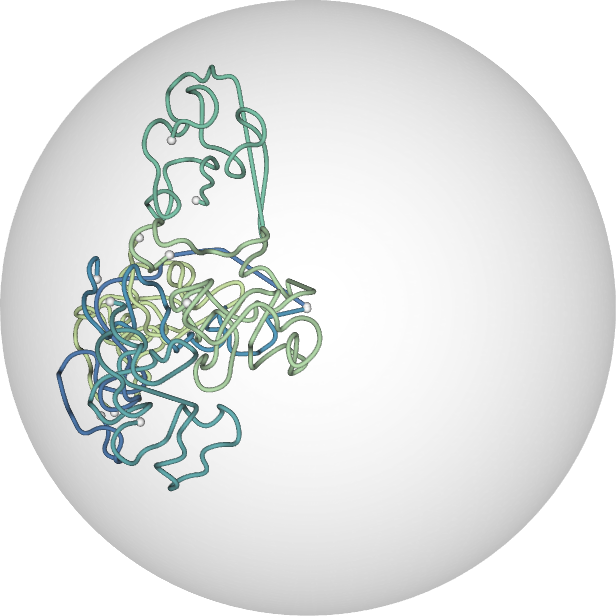
\includegraphics[width=0.3\textwidth]{\detokenize{figs/Nelle-3D/partial_1.png}}}
  \hspace{0.02\textwidth}
  \subfloat[Chromosomes
  16--22]{\label{fig:3Dp2}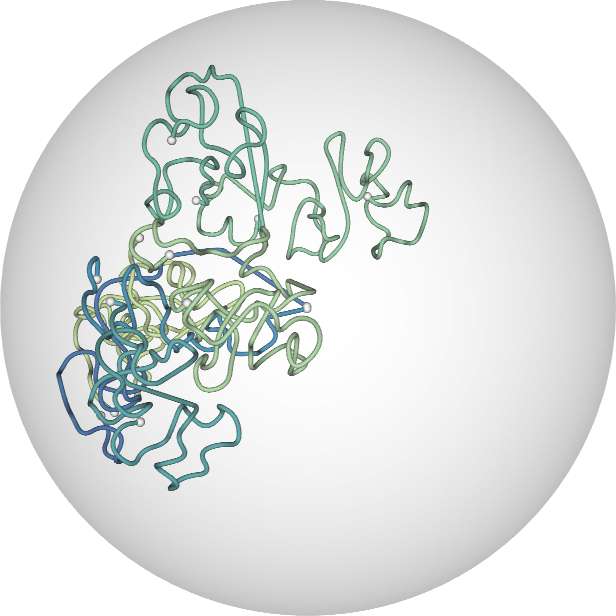
\includegraphics[width=0.3\textwidth]{\detokenize{figs/Nelle-3D/partial_2.png}}}
  \end{center}
\caption{Gene-poor chromosome 18 does not colocalize strongly with other small chromosomes that are gene-rich.}
{}
\label{suppfig:chr18in3D}
\end{figure}
\clearpage


%\begin{figure}
%\centering
%\includegraphics[width=1.0\textwidth]{suppfigs/twoPhaseMapping.pdf}
%\caption{{\bf Outline of the two-phase mapping strategy that
%captures multi-locus contacts.}
%\footnotesize{
%{\bf(a)} Further processing of each read that could not be mapped to genome as
%a whole. We count the number of cut (cleavage) sites that belong to any one of
%the restriction enzymes (REs) used in DNA digestion step for each such non-mapped
%read.  If there are only one or two such sites then we break the into smaller
%fragments (either two or three) from these sites and re-map the two longest
%fragments back to genome in the second phase. We discard from second phase
%mapping the reads that do not contain a cut site or contain more than two cut
%sites.
%{\bf(c)} Case 1: Both ends of a paired-end are fully mapped to genome in the
%first phase. Only one binary chromatin contact can be inferred.
%{\bf(d)} Case 2: One end is fully mapped but the other end cannot be mapped in
%the first phase. If the non-mapped end can be broken into smaller fragments that
%are both mapped to genome separately then a triple contact is inferred. If
%only one fragment out of the two can be mapped then a binary contact that was
%missed by the first mapping phase is inferred.
%{\bf(e)} Case 3: Both ends failed to map to genome in the first phase. If each
%end can be broken into two smaller fragments that are both mapped to genome
%separately then a quadruple contact is inferred. Remaining cases can only
%produce binary and/or triple chromatin contacts.}
%}
%\label{fig:twoPhaseMapping}
%\end{figure}
%\clearpage

% ================================================================================
% TABLES

% to make sure table captions are not centered

\captionsetup{singlelinecheck=off}
\section*{Supplementary Tables}
\begin{table}[ht!]
\caption{{\bf Sequences of primers used for PCR verification.}}
{These primers are designed to test 10 triple contacts listed in Main Figure~5
    that involve \emph{IGF2-H19} (ICR). Individual
    paired-end reads that produced each triplet are analyzed to construct
    forward/reverse primer pairs that are upstream/downstream of the MboI
    junction site that resulted in the corresponding chimera. All primer
    sequences are reported in $5'$ to $3'$ orientation even though
    reverse complements are used for reverse primers. The ``Expected sizes''
    column lists the PCR products that are expected to be amplified
    when each primer triple is used.}
\vspace{10pt}
\small{
\begin{center}
\begin{tabular}{lccccc}
\hline
\multirow{2}{*}{Label} & \multirow{2}{*}{Chr.} & {Dist. to } & \multirow{2}{*}{Primer sequence} & \multirow{2}{*}{Strand} & {Expected} \\
& & junction & &  & sizes (bp) \\\hline
%1
1a & 11 &  +44  & $5'$-GTGACTGTGAACATTTTAACATGCATGTTTAACGC-$3'$ & forward & \multirow{3}{*}{86, 90} \\
1b & 11 &  -42  & $5'$-TGCTGCACCCACATTAGCAGATTATCTCA-$3'$ & reverse & \\
1c & 17 &  -46  & $5'$-AGGGTGATTTTCTTACTGTTTGTAAATAGTGCC-$3'$ & reverse &  \\\hline
%2
2a & 8 &  +121  & $5'$-AGGTGGTAGTCAGAGAATCAGTAAAG-$3'$ & forward & \multirow{3}{*}{142, 212} \\
2b & 11 &  +51  & $5'$-TATAAGCCAAGGAGAGAGGCCTTGGAG-$3'$ & forward & \\
2c & 11 &  -91  & $5'$-ACCCTTTCTCTTTTCCCCATTGGTGGTG-$3'$ & reverse &  \\\hline
%3
3a & 11 &  -73  & $5'$-TGTGAGCTGGTGCCAAGGACAGAGGCATCA-$3'$ & reverse & \multirow{3}{*}{112, 124} \\
3b & 11 &  -39  & $5'$-CTCTTCCTTTTGGGGTGAAGACTGTCACCTTCTG-$3'$ & reverse &  \\
3c & 11 &  +51  & $5'$-ATTCAGAGGCATGACAGTCTCAAGTTCTTGGGA-$3'$ & forward & \\\hline
%4
4a & 11 &  -61  & $5'$-TTGGCCACGGGCTCTGGAGGCCAGTGCCT-$3'$ & reverse & \multirow{3}{*}{135, 140} \\
4b & 4 &  +74  & $5'$-GTAGGGAGGGAGAAACGGTAATGCTGGTCA-$3'$ & forward & \\
4c & 11 &  +79  & $5'$-GGAGGCTCAGGTGAGCCCAGGTCTCCCTCTC-$3'$ & forward &  \\\hline
%5
5a & 11 &  -131  & $5'$-CACCATCCTCCCTCCTGAGAGCTCATTCACTCC-$3'$ & reverse & \multirow{3}{*}{179, 206} \\
5b & 11 &  +48  & $5'$-GCAGCAGTGGCGCTCCCAGCTCTTTAGCA-$3'$ & forward & \\
5c & 11 &  +75  & $5'$-TCGTAGGAGACTTTCACGGAGTGCCTGGTCTCC-$3'$ & forward &  \\\hline
%6
6a & 2 &  +61  & $5'$-GCTTATTCTCCATCGGTTTCTAAAGTTGTTCAT-$3'$ & forward & \multirow{3}{*}{96, 123} \\
6b & 11 &  -62  & $5'$-ATTTCATCTCTGACCCAACCAATCAGCACTCCCTA-$3'$ & reverse & \\
6c & 4 &  +35  & $5'$-ATTGTTTCCCAGTTCTGGAGTCCAGAAGTCCAA-$3'$ & forward &  \\\hline
%7
7a & 11 &  +73  & $5'$-TGCTTGCTCCTCCGGATGTCCCCTGTGTTTT-$3'$ & forward & \multirow{3}{*}{130, 145} \\
7b & 5 &  +88  & $5'$-CCCAAAGTCATTGATATGGTTTGGCTGCATGTC-$3'$ & forward & \\
7c & 5 &  -57  & $5'$-TGCTGATGAATATCTTGGCATCTAGGGGTCAAA-$3'$ & reverse &  \\\hline
%8
8a & 5 &  +47  & $5'$-CAGAAGTTAGGAGAGTCTTGAGTGTGCCTGTTT-$3'$ & forward & \multirow{3}{*}{154, 171} \\
8b & 11 &  +74  & $5'$-TGTGGGCAAATTCACCTCTCCACGTGCCAACTA-$3'$ & forward & \\
8c & 15 &  -97  & $5'$-AAAAATATGTTTCCCAGAAACTAGAGACTGGAG-$3'$ & reverse &  \\\hline
%9
9a & 7 &  +61  & $5'$-TGCCCATAGAAACAATTTACTCCAAGGGTCAAT-$3'$ & forward & \multirow{3}{*}{98, 110} \\
9b & 11 &  +49  & $5'$-ACACCCGAGCCATCGAACATCCTAACCCCATCA-$3'$ & forward & \\
9c & 5 &  -37  & $5'$-AGCACATGCTAATGCTATCATGAAGTCATACAC-$3'$ & reverse &  \\\hline
%10
10a & 8 &  +55  & $5'$-CCTCTTGTATTTGCTTTTTCCTCTTATCTCTCT-$3'$ & forward & \multirow{3}{*}{113, 119} \\
10b & 11 &  +49  & $5'$-ACACCCGAGCCATCGAACATCCTAACCCCATCA-$3'$ & forward & \\
10c & 12 &  -64  & $5'$-TCCCTCTCTCTTTTGTTTTTTGTACTTTATTTG-$3'$ & reverse &  \\\hline
\end{tabular}
\end{center}
}
\label{supptable:PCRprimers}
\end{table}
\clearpage

\section*{Description of additional data files}
\vspace{20pt}

  {
  \subsection*{Additional file 2 --- Summary of the two-phase mapping results (XLSX).}
  This file contains separate worksheet describing in detail the numbers of reads
  processed at each step of our two-phase mapping.
  }
  \subsection*{Additional file 3 --- Rotating view of our KBM7 3D model (MP4).}
  This file contains a movie of the KBM7 3D structure that resulted in the highest log
  likelihood inferred by our algorithm. Each chromosome is colored as indicated in
  Figure~\ref{fig:3D}b.



